%%%%%%%%%%%%%%%%%% USAGE INSTRUCTIONS %%%%%%%%%%%%%%%%%%
% - Compile using LuaLaTeX and biber, unless there is a particular reason not to. Do not use the older LaTex/PDFLaTeX or BibTeX. (The fonts won't work correctly.)
% - Font and the report 'year' must be specified when all \documentclass or the template won't work correctly. (There's no error checking/default cases!)
% - For best performance save images/graphics as PDF files, not as png/jpg/eps. This makes no difference to how images are inserted using \includegraphics.
% - As many further packages as wanted can be loaded. Below are just an example set. Note that template itself loads a number of packages, including hyperref.
% - References are handed using biblatex.
% - Link to the presentation of theses policy: https://documents.manchester.ac.uk/DocuInfo.aspx?DocID=2863

%%%%%%%%%%%%%%%%%% META DATA SETUP %%%%%%%%%%%%%%%%%%
% This is where the document title and author are set. Other details for the title page are set later
% Note that if/when you edit these you may need to 'Recompile from scratch' to get the changes to display in the PDF. (In Overleaf, select the down arrow to the right of the 'Recompile' button)

    \begin{filecontents*}{\jobname.xmpdata}
        \Language{en-GB}
        \Copyrighted{True}
        % More meta-data fielda can be added here if wanted, see https://ctan.org/pkg/pdfx?lang=en for fields
    \end{filecontents*}

    %%%%%%%%%%%%%%%%%% DOCUMENT SETUP %%%%%%%%%%%%%%%%%%
    \documentclass[12pt]{uom_eee_dissertation_casson} 
    %%%%%%%%%%%%%%%%%% PACKAGES AND COMMANDS %%%%%%%%%%%%%%%%%%
    % Packages
    \usepackage{graphicx,psfrag,color} % for postscript graphics files
        \graphicspath{ {./images/} }   % where to look for images
    \usepackage{amsmath}               % assumes amsmath package installed
        \allowdisplaybreaks[1]         % allow eqnarrays to break across pages
    \usepackage{amssymb}               % assumes amsmath package installed 
    \usepackage{url}                   % format hyperlinks correctly
    \usepackage{rotating}              % allow portrait figures and tables
    \usepackage{multirow}              % allows merging of rows in tables
    \usepackage{lscape}                % allows pages to be typeset in landscape mode
    \usepackage{tabularx}              % allows fixed width tables
    \usepackage{verbatim}              % enhanced version of built-in verbatim environment
    \usepackage{footnote}              % allows more control over footnote environments
    \usepackage{float}                 % allows H option on floats to force here placement
    \usepackage{booktabs}              % improve table line spacing
    \usepackage{lipsum}                % for adding dummy text here
    \usepackage[base]{babel}           % for proper hypthenation in lipsum sections
    \usepackage{subcaption}            % for multiple sub-figures in a single float
    % Add your packages here
    %\usepackage{pdfcomment}            % for alt text for accessibility
    \usepackage{booktabs}              % for better looking tables
    % Then to add images use:
    % \pdftooltip{\includegraphics[width=0.5\textwidth]{image.pdf}}{Alt-text here}
    % This makes the text in the image non-select-able though (assuming it's a vector file)
    
    % Custom commands
    \newcommand{\degree}{\ensuremath{^\circ}}
    \newcommand{\sus}[1]{$^{\mbox{\scriptsize #1}}$} % superscript in text (e.g. 1st)
    \newcommand{\sub}[1]{$_{\mbox{\scriptsize #1}}$} % subscript in text
    \newcommand{\sect}[1]{Section~\ref{#1}}
    \newcommand{\fig}[1]{Fig.~\ref{#1}}
    \newcommand{\tab}[1]{Table~\ref{#1}}
    \newcommand{\equ}[1]{(\ref{#1})}
    \newcommand{\appx}[1]{Appendix~\ref{#1}}
    %%%%%%%%%%%%%%%%%% REFERENCES SETUP %%%%%%%%%%%%%%%%%%
    % Setup your references here. Change the reference style here if wanted
    \usepackage[style=ieee,backend=biber,backref=true,hyperref=auto]{biblatex}
    % Note backref=true adds a page number (and hyperlink) to each reference so you can easily go back from the references to the main document. You may prefer backref=false if you need to stick strictly to a given reference style
    % Fixes which can't be applied in the .cls file
    \DefineBibliographyStrings{english}{backrefpage = {cited on p\adddot},  backrefpages = {cited on pp\adddot}}
    %  \renewcommand*{\bibfont}{\large}
    % Add more .bib files here if wanted
    \addbibresource{references.bib }
    
    %%%%%%%%%%%%%%%%%% START DOCUMENT %%%%%%%%%%%%%%%%%%

    \begin{document}
    \makeatletter
    \title{Development of Two Wheel Self Balancing Line Following Robot} % title of your thesis
    \author{Winston Scott}
    \studentid{107067151}
    \makeatother                                               
    \wordcount{1000}		                    % use \wordcount{} to set the count, \thewordcount to print in the text
    \maketitle

    %%%%%%%%%%%%%%%%%% LISTS OF CONTENT %%%%%%%%%%%%%%%%%%
    \uomtoc
    \begin{uomterms}
        \textbf{TWSB}:Two Wheel Self Balancing \\
        \textbf{DDMR}:Differential Drive Mobile Robot \\
        \textbf{LQR}:Linear Quadratic Regulator \\
        \textbf{MEMS}:Micro-Electro-Mechanical Systems \\
        \textbf{MPC}:Model Predictive Control \\
        \textbf{MCU}:Microcontroler Unit \\
        \textbf{RPC}:Remote Procedure Call \\
        \textbf{IMU}:Inertial Measurement Unit \\
        \textbf{ppr}:Pulses Per Revolution \\
        \textbf{KF}:Kalman Filter \\
    \end{uomterms}

    %%%%%%%%%%%%%%%%%% ABSTRACT %%%%%%%%%%%%%%%%%%
    \begin{abstract} % put abstract here. Limit is 1 page.
    The highly dynamic Two Wheel Self Balancing Robot 
    (TWSB) has a large exploration space for developing high level 
    control strategies. 
    This report presents the design decisions and algorithms developed for
    an autonomous line racing TWSB robot utilizing a monocular vision system with low cost hardware. 
    System identifications techniques are used to explore
    cascaded PID and LQG control strategies.
    A trajectory generation algorithm is proposed based on drivability, confidence 
    and prominence of the detected line from a camera used as an intensity sensor. 
    The performance of the the system is shown to be robust to different race tracks which
    surface texture variation, lighting conditions, high speed straights and tight curves. 


  \end{abstract}%
  \clearpage

  \uomdeclarations

  %%%%%%%%%%%%%%%%%% SECTION 1 %%%%%%%%%%%%%%%%%%
    \section{Introduction}
    The Two Wheel Self Balancing (TWSB) system is a nonlinear, underactuated system that is dynamically stable.
    Compared to the differential drive mobile platform (DDMR), the TWSB requires active control effort
    to maintain its upright posture while in motion and when stationary.
    Substantial research, has been conducted on the similarly unstable 1-DOF inverted pendulum on a cart 
    as a benchmark for control techniques \cite{boubaker2013inverted}. 
    The TWSB robot serves as a cost-effective platform for research and education in complex control 
    strategies less commonly applied statically stable wheeled robots \cite{educationPlatform}.
    
    Controlling this unstable degree of freedom expands the range of autonomous behaviors that 
    can be explored \cite{RoboLimbo} \cite{jeong2008wheeled} \cite{Browning2004TurningSI}. 
    These behaviors necessitate a hierarchical design in the system's architecture,
    where planning and navigation algorithms though linked, are decoupled by levels of abstraction 
    from the low-level stability control and even lower level motor control.
    
    A notable work on the TWSB system is \cite{grasser2002joe} which designed a TWSB robot capable of disturbance
    rejection and static stability on an inclined plane. This was achieved using an FPGA-based DSP system, 
    and by decoupling the balancing and steering torques in state space an optimum Linear Quadratic Regulator (LQR). 
    Intuitive references of linear velocity and angular rate are used for teleoperation. An early challenge in the navigation of the TWSB system 
    identified by \cite{SelfContainedMobileTWSB} is the sensor system used for state estimation. The proposed solution 
    maintains a running sum of the gyroscope as a augmented state variable in the form of a slowly monotonically increasing function of the gyroscope's bias.

    Advances in the cost-to-performance of embedded systems and micro-electromechanical sensors (MEMS) \cite{MEMS} 
    have allowed \cite{juang2013design} \cite{Velazquez2016VelocityAM} to remotely control the TWSB system 
    using low-powered microcontrolers. This is accomplished through a cascaded PID controller, 
    similar to those employed in quadrotor control.
    
    Recent research has also applied reinforcement learning to the TWSB system \cite{kober2013reinforcement}.
    Neural networks are proposed as nonlinear function approximations to model the system's dynamics. 
    These methods demonstrate robustness to un-modeled dynamics \cite{guo2021optimal}. By utilizing 
    brushless motors that lend themselves to torque control in direct drive systems, the TWSB’s pitch 
    angle can be regulated via a PID controller, minimizing positional drift caused by backlash-induced 
    vibrations when balancing.
    
    In mobile robotics, the ability to navigate requires perception. LIDARs are commonly used, as  
    the information they capture naturally lends itself to path-planning algorithms [].
    Another commonly used multimodal sensor is the CMOS camera, which measures light intensity at each pixel. 
    When paired in stereo, it can efficiently infer depth [], providing a suitable alternative to the point 
    clouds generated by LIDAR. Although monocular vision systems are desirable due to their simplicity, 
    the redundancy of stereo vision proves beneficial in safety-critical applications [].
    Both sensors provide rich environmental data that can be leveraged to develop long-term path-planning algorithms.
    
    This paper presents the design of a TWSB robotic platform capable of autonomously navigating an 
    indoor line track. The line is assumed to be of significant contrast to the environment, with computer 
    vision algorithms used to locate it. A racing algorithm is proposed,
    based on three key metrics of the line: drivability, confidence, and prominence.
    \cite{visionlinetwsb} utilizes a camera as a matrix of binary intensity sensors and a rule-based 
    algorithm to follow a line while balancing. A similar approach by \cite{ghani2011two} uses infrared sensors. 
    \cite{nntwsbvision} trained an end-to-end neural network to perform the same task, while [] proposes a 
    convolutional neural network-based method that uses RDB-Depth camera data to autonomously 
    navigate with human-centric social behavior. Similarly, [] develops planar-wheeled robot navigation 
    algorithms through lane segmentation using geometric computer vision techniques.
    While considerable success has been achieved by obtaining a linear approximation of the dynamics in a similar fashio to 
    of the classic inverted pendulum, \cite{AdvancedWIP} explores the use of non-linear control strategies, such as backstepping or 
    sliding mode control. An online data-driven model of a mobile system and embeds it 
    in a Model Predictive Controller (MPC). This adaptive control strategy is robust to the un-modeled 
    environment and plant dynamics, allowing for autonomous aggressive maneuvers along a mapped track.
    
    This project develops a TWSB robot capable of autonomously navigating a line track.
    The platform is demonstrated as a cost-effective solution providing foundation for further research in mobile robotics.
    Autonomy is achieved using a stabilizing feedback controller, with cascaded PID and 
    LQR control strategies explored for balancing and stabilizing the robot's position. 
    Once these requirements are met, the robot can be teleoperated intuitively via a 
    smartphone-based web interface. The remainder of this paper focuses on incorporating 
    multimodal sensor data from the camera to develop line-racing algorithms.
    The robot algorithmically infers and follows an unknown line using a monocular camera. 
    A hardware-in-the-loop software architecture is implemented, enabling telemetry data and control 
    commands to be exchanged between the robot and a remote computer. Visualization of this telemetry
    data provides a straightforward means of validating the robot's performance.
    \pagebreak{}

  %%%%%%%%%%%%%%%%%% SECTION 2 %%%%%%%%%%%%%%%%%%
    \section{Mathematical Modeling} % edit section heading as appropriate
    \subsection{DC Motor Model}    
    \begin{figure}[H]
        \centering
            \includegraphics[width=0.75\textwidth]{Diagrams/DcMotorModel.pdf}
        \caption{Gearbox DC Motor Model Diagram}
    \end{figure}
    The system is driven by two independently voltage controlled DC motors through 
    planetary gearboxes, as is shown in Fig(2). 
    DC motors execute a torque $t_r$, proportional to the armature current $i_a$,
    when a voltage $V_a$ is applied.
    The ratio of motors inductance $L_a$ and resistance $R_a$ determine the
    time constant $\tau_e$ of the motor. That is the time it takes 
    for $i_a$ to reach 63.2\% of its final value. []
    The gear ratio, $n=N_2/N_1$ transmits the torque to the wheel, 
    where $N_1$ and $N_2$ are the number of teeth on the input and output gears respectively.
    The equivalent viscous damping 
    $B_G$ and the moment of inertia $J_G$ with respect to the motor are given by
    \begin{equation}
        J_{\text{eq}} = J_G + J_r \cdot n^2 
    \end{equation}
    With $J_r$ representing the moment of inertia of the the rotor.

    The speed of the gearbox, $\dot\phi_w$ is related to the armature voltage 
    by the well-known transfer function
    \begin{equation}
        \begin{aligned}
            \frac{\Omega_w \left(s\right)}{V_a \left(s\right)}=\frac{K_t }{s^2 \cdot L_a R_a +\;s\left(R_a \cdot J_{\mathrm{eq}} +B_{\mathrm{eq}} \cdot L_a \right)+K_t {\cdot K}_e +R_a \cdot B_q }\cdot\frac{1}{n}
        \end{aligned}
        \label{eq:DCMotor}
    \end{equation}
    Where $\Omega_w$ is the laplace transform of the output speed, 
    The rotors viscous damping $B_r$ is assumed to be negligible, as is $B_G$. 
    For small motors, $\tau_e$ is small and $L_a << R_a$, hence the motor can be 
    approximated as a first order system as
    \begin{equation}
        \begin{aligned}
            \frac{\Omega_w \left(s\right)}{V_a \left(s\right)}=\frac{K_t }{s\cdot R_a + J_{eq}+K_t K_e }\cdot\frac{1}{n}
        \end{aligned}
        \label{eq:DCMotorSimple}
    \end{equation}

    Where $K_t$ is the torque constant of the motor and $K_e$ is the back EMF constant.
    The parameters of the motor are identified and discussed in section 3.1. 
    \pagebreak{}

    \subsection{2DOF System Model}
    \begin{figure}[h]
        \centering
        \begin{subfigure}[b]{0.4\textwidth}
            \includegraphics[width=\textwidth]{Diagrams/WIP.pdf}
            \caption{Wheeled Inverted Pendulum}
            \label{fig:WIP}
        \end{subfigure}
        \hfill
        \begin{subfigure}[b]{0.4\textwidth}
            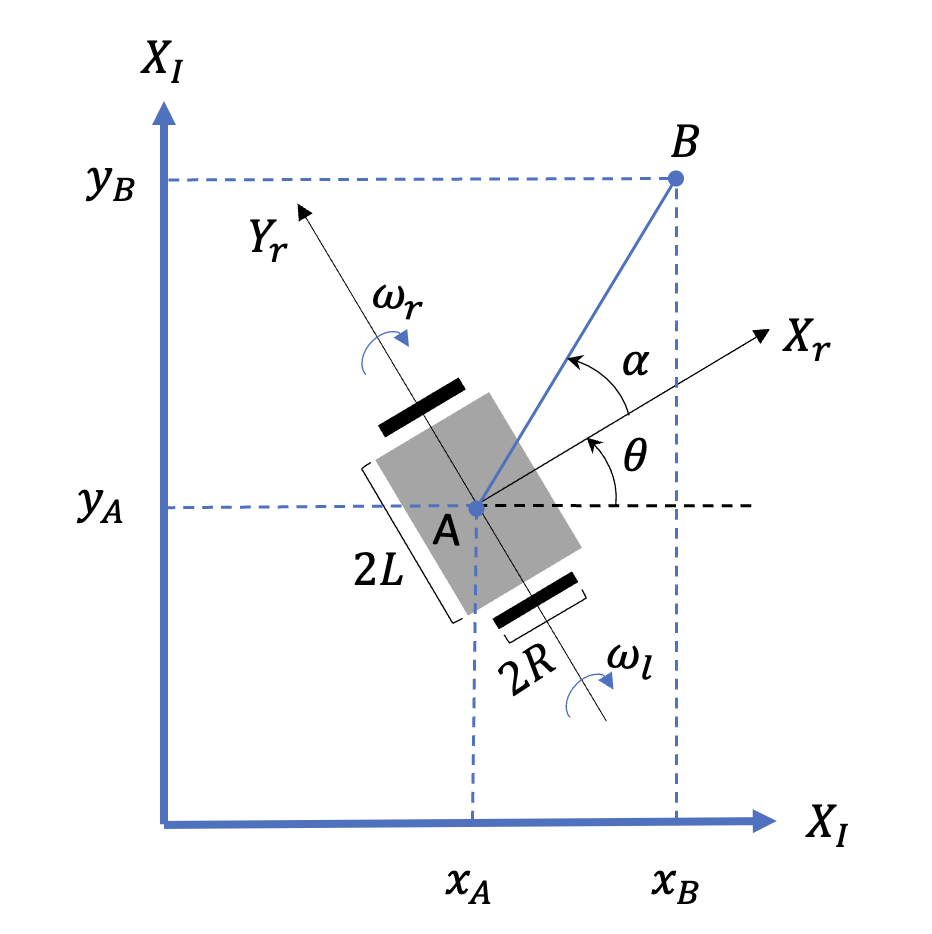
\includegraphics[width=\textwidth]{Diagrams/DDMR.pdf}
            \caption{Differential Drive Mobile Robot}
            \label{fig:DDMR}
        \end{subfigure}
        \caption{Robot motion decoupled by levels of abstraction}
        \label{fig:2DOF}
    \end{figure}

    Wheeled mobile robots are typically restricted to navigation in the 2D Cartesian plane, their motion models are often simplified and 
    abstract the non linear dynamics of friction and acceleration is assumed to be constant. 
    Effective control and planning algorithms for such platforms require the designer to obtain a mathematical model, 
    the differences in models arise form the nature of the goal of the planner, the available control signals and the sensors 
    used to estimate the configuration of the robot \cite{ClassificationWheeled}. 
    In this paper, the TWSB decomposed into 2 commonly studied 2DOF systems, as in Fig.\ref{fig:2DOF} and their behavior is analyzed
    seperately.
    
    The DDMR modeled in Fig.\ref{fig:DDMR} navigates under the pure rolling assumption, that is, the wheels do not slip 
    and the inerial forces arising from acceleration in the $x'$ direction are negligible \cite{KinematicWheeled}. 
    The motion of the DDMR is bounded by its non-holonomic constraints[], that is no lateral motion is allowed along the $y'$ axis. 

    The  DDMR's non linear kinematic model in the global frame is 
    \begin{equation}
        \begin{bmatrix}
            \dot{x}_b \\
            \dot{y}_b \\
            \dot{\theta}
        \end{bmatrix}
        =
        \begin{bmatrix}
            \frac{r}{2} \cos \theta & \frac{r}{2} \cos \theta \\
            \frac{r}{2} \sin \theta & \frac{r}{2} \sin \theta \\
            -\frac{r}{2L} & \frac{r}{2D}
        \end{bmatrix}
        \begin{bmatrix}
            \omega_L \\
            \omega_R
        \end{bmatrix}
        \label{eq:DDMR}
    \end{equation}
    Where $r$ is the radius of the wheel and $D$ is the distance between the wheels.
    from \ref{eq:DDMR} it can be seen that a large wheel radius $r$ amplifies the resultant effect of difference in the wheel 
    speeds, $\omega_L$ and $\omega_R$. This leads to very small disturbances to the wheel velocities being sufficient 
    to adequately steer the TWSB. Conversely small wheels minimize the effects of backlash in the drive train, these effects are most notable 
    when the TWSB is required to maintain static stability. \cite{kim2015dynamic} considers the dynamics of the coriolis force 
    arising from the yaw rate of the body, $\omega_b$. The robot developed in this paper is of small stature and these effects 
    are assumed to be negligible. This project is mainly concerned with the navigation the TWSB system and as such 
    relatively large wheels are used. This allows for a simplified dynamics model of the Wheel Inverted Pendulum 
    in Fig.\ref{fig:WIP} to simulate the balancing of the TWSB in 2DOF space.

    The derivation of the linearized 2DOF model for the TWSB is well known[][]. Incorporating \ref{eq:DCMotorSimple}
    with state space model obtained by \cite{Velazquez2016VelocityAM} the system in Fig.\ref{fig:WIP} is described by 
    \begin{equation}
        \left\lbrack \begin{array}{c}
        {\dot{x} }_b \\
        {\ddot{x} }_b \\
        \dot{\theta} \\
        \ddot{\theta} 
        \end{array}\right\rbrack =\left\lbrack \begin{array}{cccc}
        0 & 1 & 0 & 0\\
        0 & \frac{2n^2 K_e K_t }{r^2 R_a \cdot W_1 } & -\frac{M_b^2 L^2 g\;}{W_1 \left(J_b -M_c L^2 \right)} & 0\\
        0 & 0 & 0 & 1\\
        0 & \frac{2n^2 K_e K_t }{r^2 R_a \cdot W_1 \left(\frac{J_b }{M_b }+L\right)} & \frac{{-M}_b^2 L^2 g}{W_1 \left(\frac{J_b }{M_b }+L\right)\left(\left(J_b -M_c L^2 \right)+{\mathrm{gW}}_1 \right)} & 0
        \end{array}\right\rbrack \cdot \left\lbrack \begin{array}{c}
        x_b \\
        {\dot{x} }_b \\
        \theta \\
        \dot{\theta} 
        \end{array}\right\rbrack +\left\lbrack \begin{array}{c}
        0\\
        -\frac{2{n\;K}_t }{r\;R_a W_1 }\\
        0\\
        -\frac{2n\;K_t }{r\;R_a W_1 \left(\frac{J_b }{M_b }+L\right)}
        \end{array}\right\rbrack \cdot V_a
        \label{eq:2DOF}
    \end{equation} 

    with $W_1 =2\left(-\frac{n^2 J_{\mathrm{eq}} +J_b }{r^2 }-M_w \right)-M_b +\;\frac{M_b^2 L^2 }{J_b +M_b L^2 }$ 

    \pagebreak{}

    \section{System Design}
        \begin{figure}[H]
            \includegraphics[width=\textwidth]{DesingImgs/bBot Drawing v3.pdf}
            \caption{CAD Drawing of the TWSB system dimensions in mm}
            \label{fig:CAD}
        \end{figure}

        The TWSB body is 3D printed out of PLA plastic in 3 parts for minimal assembly.
        The battery pack is quickly swappable and both it and the electronics sub assembly 
        are soft-mounted in a roll cage like housing for protection against impacts. 
        \begin{figure}[H]
            \centering
            \includegraphics[width=0.55\textwidth]{Diagrams/SystemOverview.pdf}
            \caption{System Overview}
        \end{figure}

        Two brushed DC motors are powered by an H-Bridge IC, DRV7783. 
        The STM32F411RE Microcontroler Unit (MCU) is used to control the 
        motors and monitor the 6 Axis Inertial Measurement Unit (IMU) over I2C. It communicates with the 
        Raspberry Pi 5 over UART via a custom ASCII protocol discussed in section 2.4. 
        The system is powered by a 12V nominal Li-ion Battery pack. A USB-C CC-CV charger is used for quick 
        and accessible recharging, critical for mobile robotics applications. 
        Battery voltage is monitored by the MCU and the pack is protected by a BMS and a 3A poly-fuse.
        A simple circuit adapted from \cite{chu2008designing} is used to safely load share between the battery pack and the charger.

        \subsection{Software Architecture}
        The modern standard for robotics software is the Robot Operating System 2 (ROS2) \cite{Macenski2022RobotOS}. 
        It is composed of several highly configurable applications that are designed to be manged in a distributed system.
        Distributed systems are beneficial in robotics development as they functionally decouple the software components, 
        enabling robust failure recovery and ease of integrating new features. This is useful for this project as 
        the core control and vision systems are developed in parallel. The controls, logs and error recovery systems mandating 
        high availability compared to user interfaces such as the remote control webapp. 
        Whilst this is a powerful tool, it is deemed too complex to learn for meeting the project deadline.
        Nevertheless some core concepts are used such as sharing state by message passing between components, 
        and dynamic parameter configuration to improve testing and data collection. The ZeroMQ middleware is used for 
        timestamped signal stream communication between the computational nodes shown in Fig.\ref{fig:DataPath}.
        \begin{figure} [H]
            \includegraphics[width=\textwidth]{Diagrams/CommunicationDataPath.pdf}  
            \caption{Communications Data Path, borders show where state is shared}
            \label{fig:DataPath}
        \end{figure}

        The software, written in C++, is managed by systemd as services. 
        Self-diagnosis routines are used for resource monitoring and auto recovery. 
        Programs operate on runtime parameters through Remote Procedure Call (RPC) 
        interface using a GET-SET pattern. This reduces the 
        compile flash debug iteration time. A GStreamer pipeline sets up a video 
        server accessible over LAN. OpenCV is used for optimized image processing.
      
        The firmware is implemented in C using register definitions from the 
        libopencm3 project \cite{BeginningSTM32} as an exercise in low level programming. 
        No dynamic memory allocation is used.
        The resultant binary is 19KB with 892B of RAM used.
        A simplified sprintf function from [] is the only external dependency.
        The MCU also presents the same RPC interface over uart serial link.
        This executes commands and publishes telemetry at 100Hz.

        The data-acquisition system obtains a timestamped sample of the 
        telemetry values transmitted by the MCU through a serial link.
        This can result in non-uniformly sampled data as parsing the UART IO buffer 
        is constrained by the OS scheduler, thus an event driven system is used to 
        minimize CPU overhead. Worst case jitter is observed, under CPU stress 
        tests to be 0.1ms. This is acceptable for telemetry data. 
        \pagebreak{}
        \subsubsection{Parameters }
        The system parameters are given in table(1). 
        The mass of the sub-components obtained by weighing,
        and estimates of the 3D printed parts mass are given by the slicer software. 
        The CAD files are used in MATLAB's Multibody Simulink environment, which 
        computes the center of mass and the moments of inertia.
        The Motor parameters and estimated as per [] using the manufacturers dataset[] summarized in table(2).
    
        \begin{table} [H]
            \centering
            \begin{tabular}{|c|c|c|c|}
                \hline
                Parameter & Value & Units & Description \\
                \hline
                $m$ & 1.5 & kg & Mass of the body \\
                $l$ & 0.1 & m & Length of the body \\
                $J_b$ & 0.01 & $kgm^2$ & Moment of inertia of the body \\
                $r$ & 0.03 & m & Radius of the wheel \\
                $d$ & 0.132 & m & Wheel base \\
                $R_a$ & 1.5 & $\Omega$ & Resistance of the motor \\
                $K_t$ & 0.01 & Nm/A & Torque constant of the motor \\
                $K_v$ & 0.01 & V/rad/s & Back EMF constant of the motor \\
                $J_w$ & 0.01 & $kgm^2$ & Moment of inertia of the wheel \\
                \hline
            \end{tabular}
            \caption{System Parameters}
        \end{table}



        \pagebreak{}

        \subsection{System Identification}
        A set of experiments are conducted to obtain an estimate transfer function of the motors.
        \begin{table}[H]
            \centering
                \begin{tabular}{|r|c|c|c|c|c|c|}
                    \hline 
                    Gear Ratio & Rated Torque & Rated Speed  & Rated Current & Stall Current & Stall Torque \\
                    \hline
                     1:20  & 0.39 Nm & 600 rpm & 500 mA & 2 A & 0.15 Nm/Kg \\
                    \hline
                \end{tabular}
                \caption{Manufacturer Provided Motor Parameters}
        \end{table}
        A telemetry and analysis software system developed in python. It is used as 
        test bench  setup shown in Fig.\ref{fig:SysIDSetUp}, a series of reference 
        ramp, step, sine and chirp inputs are applied to each motor, 
        the resultant input outputs are shown 
        in Fig.\ref{fig:openloop}.
       
        \begin{figure}[H]
            \centering
            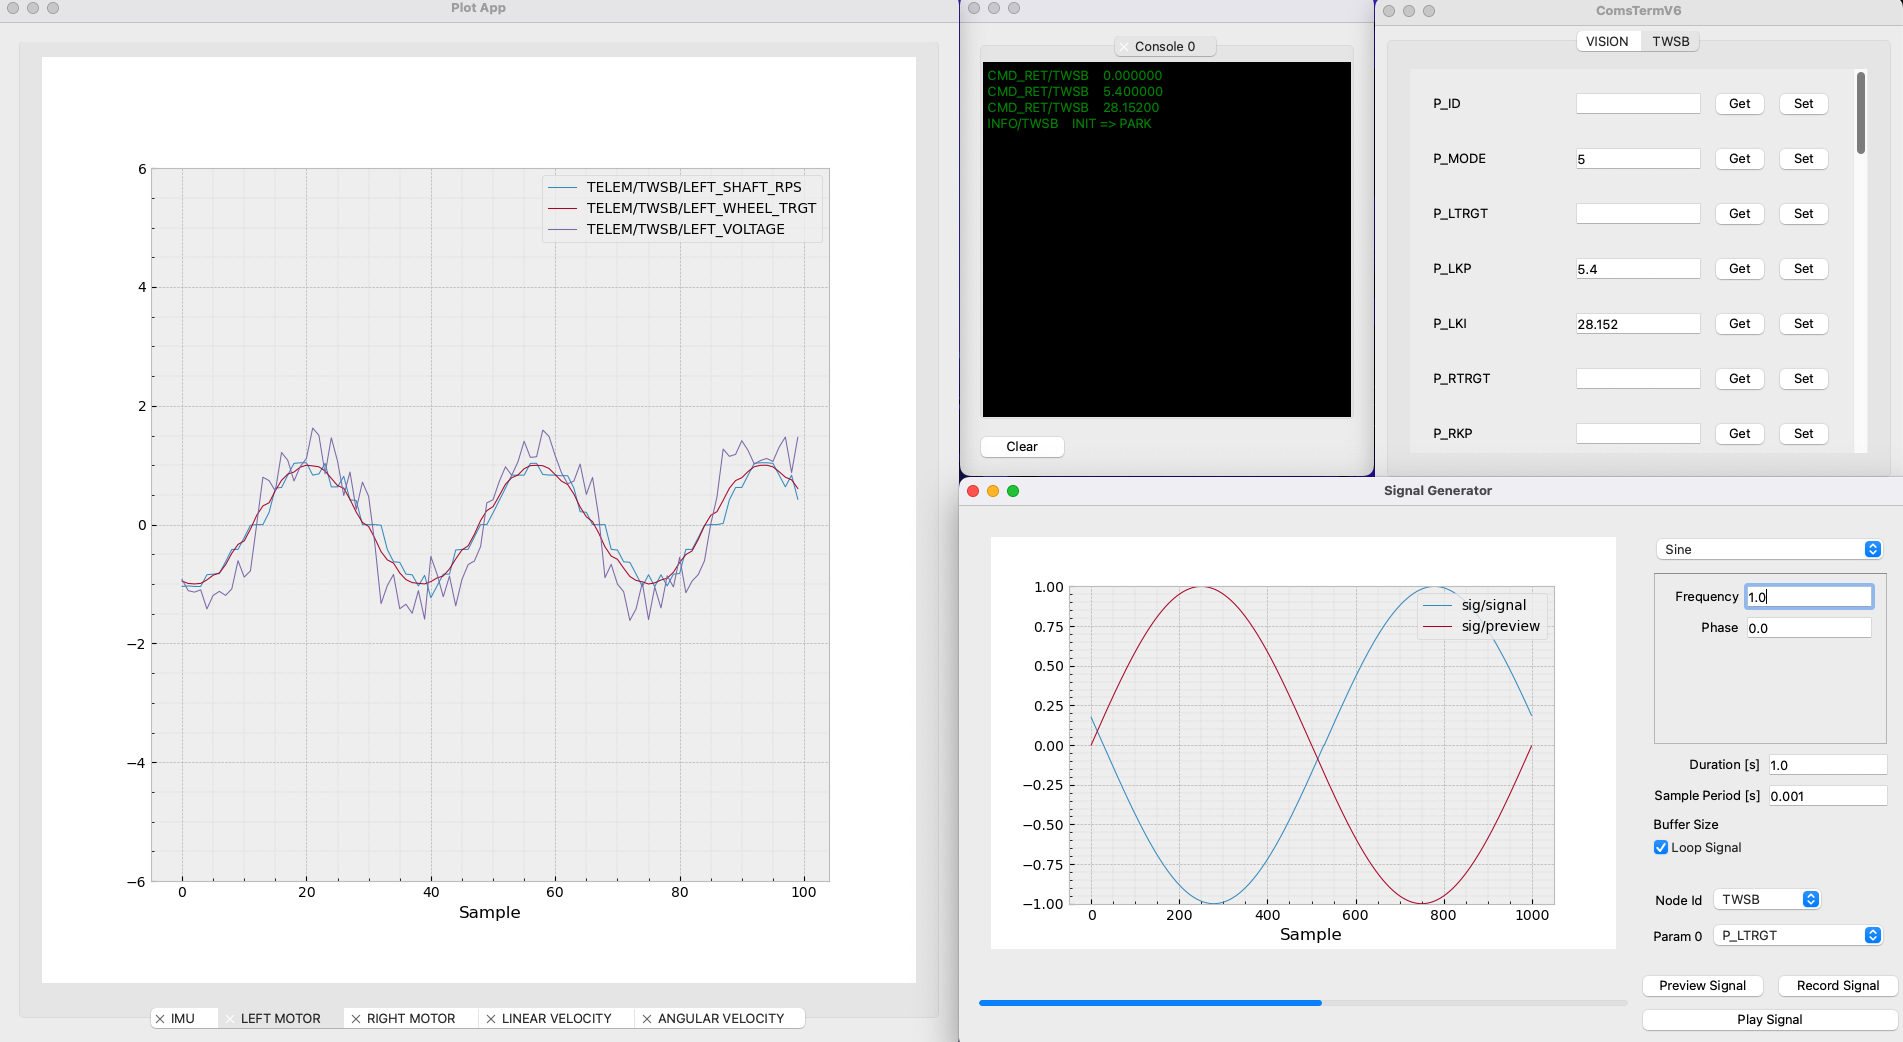
\includegraphics[height=0.\textwidth]{SysIDMotorSetUp.png}
            \caption{System Identification Testbench Setup}
            \label{fig:SysIDSetUp}
        \end{figure}
        The test suit contains a timeseries signal generators, with preview and playback functionality.
        The Systems logs and messages are displayed in a terminal window, and the user is able to fully configure 
        each nodes runtime parameters remotely over a network connection, utilizing the RPC ASCII protocol.
        A line plotter, is configured by JSON to display any number of signals.
        This architecture allows for repeatability in obtaining robot data, something 
        is is a challenge in mobile robotics[]. 
        
        This software system is also utilized for huristic tuning of the control
        and vision systems. The program is able to visualize control signal streams in soft real time, 
        and provides a useful insight into the effects of the control system on the plant.

        \begin{figure}[H]
            \centering
            \begin{subfigure}[b]{0.45\textwidth}
            \includegraphics[width=\textwidth]{Graphs/openstep.pdf}
            \caption{Open Loop Step Response}
            \label{fig:openstep}
            \end{subfigure}
            \hfill
            \begin{subfigure}[b]{0.45\textwidth}
            \includegraphics[width=\textwidth]{Graphs/1HzSine.pdf}
            \caption{Open Loop Sine Response}
            \label{fig:opensine}
            \end{subfigure}
            \caption{Open Loop no Load Speed Voltage Experiments}
            \label{fig:openloop}
        \end{figure}


        From these experiments it is clear that the motor is has significant deadzones, 
        and the input output relationship is non linear at low speeds. When the motor is operating at its rated currnet, 
        seen by the experiments in Fig.\ref{fig:speedvolt}, its its linearity is improved. The maximum no load speed is  
        \begin{figure}[H]
            \centering
            \includegraphics[width=0.5\textwidth]{Graphs/SpeedVoltageCurve.pdf}
            \caption{Speed Voltage Relationship}
            \label{fig:speedvolt}
        \end{figure}

        This non-linearity is a result of the motors backlash, which is a common issue in low cost gearboxes.
        \cite{grasser2002joe} utilizes a low pass filter to mitigate some of the more sever effects of 
        this deadline; mechanical vibration increased thermal stress and noise. 
        In the case of the TWSB system, when it is stationary, 
        the actuators will not be static and are required to be operating mostly is a sinusoidal version, 
        similar to Fig.\ref{fig:opensine} in order to regulate the pitch angle of the body.
        Considering this a closed loop controller is developed in section 4.1 to regulate the motors speed,
         and maintain the device is it operating region. 
    \pagebreak{}



    \section{State Estimation}
    Information about the TWSB system may be obtained from 2 kinds of sources; 
    mathematical models models as in eq(1) which can describe the time evolution of the chosen system variables, 
    and sensors that convert energy arising from a physical property into information. Both of these sources 
    are approximations of the true state. The process of combining multiple sources of information is termed sensor fusion.
    This section evaluates the available methods employed using \textit{proprioceptive} sensors.
    \subsection{Sensors Overview}
        For the TWSB system in eq(\ref{eq:2DOF}) its state variables $\theta$ and $\dot x_b$ can be measured through the onboard IMU 
        and the wheel encoders respectively. 
            
        The motors incorporate a low-cost 12 pulses per revolution (PPR) incremental encoder on the rotor shaft. 
        Further resolution is easily obtained by using the hardware quadrature decoder 
        peripheral to increment, or decrement, a counter based on the direction of movement. 
        Considering the gearbox ratio $n=20$ results in an effective resolution of 960 PPR. 
        The rotational speed of the wheel is computed by sampling the change in the pulse counts
        at a fixed rate as per 
            \begin{equation}
                \omega=2\pi \frac{\Delta \textit{count}}{PPR \cdot \Delta t}
            \end{equation}
    
        Where $\Delta \textit{count}$ is the change in the pulse count. The sample period is inversely proportional to the
        quantization error in the velocity estimate. 
        However, it is observed that larger sources of error arise from the mechanical backlash in the gearbox.
        The sample time is set to 2ms, and a low-pass filter is given by the recursive relation
            \begin{equation}
        y_k = \alpha x_k + (1-\alpha)y_{k-1}
                \label{eq:lpf}
            \end{equation}
        Selecting $\alpha = 0.95$, attenuates exponentially sudden deviations in the velocity estimate.

        Utilizing this velocity in the model of the DDMR in eq(\ref{eq:DDMR}) to obtain the
        position of the robot in the cartesian plane as ($x_g,y_g$)is known as odometry.
        There are various sources of errors in 
        this process, arising from assembly imperfections and conditions in 
        the environment which may break the constraints assumed in the kinematics of the DDMR.
            
        These conditions become significant in the case of the TWSB system as crashes, or bumps, result in large 
        and unbounded error accumulation. In the case of crashes, the robot is subsequently stationary 
        and its state is reset. However, in the case of bumps, where the robot can recover, corrective 
        action is required to mitigate this. Assuming a sufficiently accurate wheel encoder, a simple method is 
        implemented based on \cite{Gyrodometry}, only correcting 
        the odometry when such events are detected.  
        This leads to the decision that other forms of systematic odometry errors have to be 
        either disregarded in the short term or corrected by landmark methods by $exteroceptive$ sensors. 

        The IMU is a 6 axis MEMS sensor[] which measures the local linear acceleration 
        and angular velocity.
        The 3D acceleration $\vec{a}$ is used to obtain an 
        estimate of the pitch angle as    $\hat{\theta} = \mathrm{atan2}\left(-a_x ,a_z \right)$

        The variance of this $\hat{\theta}$ is small when the system is at rest, but grows larger when subject to vibration from the motors
        as shown by the experiment in Fig.\ref{fig:accelNoise} where the TWSB is placed horizontally at rest and motor control commands are issued. 
        \begin{figure}[H]
            \centering
            \begin{subfigure}[b]{0.5\textwidth}

                \includegraphics[width=\textwidth]{Graphs/accelNoiseReadings.pdf}
                \caption{Accelerometer is sensitive to motor vibrations}
                \label{fig:accelRaw}
                
            \end{subfigure}
            \hfill
            \begin{subfigure}[b]{0.45\textwidth}
                \includegraphics[width=\textwidth]{Graphs/noisyPitchEst.pdf}
                \caption{Wide Variance on pitch estimate at rest}
                \label{fig:pitchNoise}
            \label{fig:accelNoise}
            \end{subfigure}
            \caption{Accelerometer Noise}   
        \end{figure}

        From \ref{fig:pitchNoise} it can be seen that the IMU is not mounted perfectly orthogonal to the body frame. 
        \begin{table}[H]
            \centering
            \begin{tabular}{c c c} 
                \toprule
                $a_{x_0}$ & $a_{y_0}$ & $a_{z_0}$ \\
                \midrule
                0.036453 & -0.0021066 & 0.133658 \\
                \bottomrule

            \end{tabular}
            \caption{Accelerometer Mounting Offset (m/s$^{2}$)}
            \label{tab:accelOffset}
        \end{table}
        This systematic error is removed by utilizing calibrated values in table obtained as per \ref{tab:accelOffset}.
        
        
        \pagebreak{}
        \subsection{Kalman Filter}
        The Kalman Filter (KF) and its variants  are widely used in robotics to fuse 
        complementary sources of information \cite{Thrun2005ProbabilisticRobotics} \cite{perez2023quadcopter} \cite{Moore2014AGE}.
        The ordinary KF is applicable to linear systems, as a type of Bayesian filter, 
        the discreet representation of the KF represents current belief $bel(x_k)$ around the true state,
        as a Gaussian whose distribution is parameterized by its mean $\mu_k$ and covariance matrix $P_k$.

        A new measurement is observed at each timestamp through the linear function $z_k = C_k x_k + R_k$. 
        The measurement model $C_k$ is used to map the true state into the measurement space.
        Here the process and measurement noise are Gaussian with zero mean and covariance $Q_k$ and $R_k$ respectively. 
        The Kalman Gain computed as \ref{eq:KalmanGain} provides the optimal weighting between t
        he beliefs from the prediction \ref{eq:KalmanPredict} and the measurement update \ref{eq:KalmanUpdate}.
        

        \begin{subequations}
            \begin{equation}
                \bar{bel}(x_k) = \begin{cases}
                        \bar{\mu}_k = F_k \mu_{k-1} + G_k u_k \\
                        \bar{P}_k = F_k P_{k-1} F_k^T + Q_k
                        \end{cases}
                \label{eq:KalmanPredict}
            \end{equation}
            \begin{equation}
                K_k = \bar{P_k} C_k^T \left(C_k \bar{P_k} C_k^T + R_k \right)^{-1}
                \label{eq:KalmanGain}
            \end{equation}
            \begin{equation}
            bel(x_k) = \begin{cases}
                \mu_k = \bar{\mu}_k + K_k \left(z_k - C_k \bar{\mu}_k \right) \\
                P_k = \left(I - K_k C_k \right) \bar{P}_k
            \end{cases}
            \label{eq:KalmanUpdate}
            \end{equation}
            \label{eq:KalmanAlgorithm}
        \end{subequations}
     
        Even though the state transition model of the TWSB robot is non-linear
        \cite{ooi2003balancing} 
        developed self balancing platforms capable of restricting oscillations about the 
        operating point to $±1$ degree. This one order of magnitude than the worst case pitch limit of $±10$ degrees.
        Beyond this, the small angle approximation is no longer valid, and the system is not locally linear. 

        The state transition model used by the KF, can be choses to model the TWSB system \ref{eq:2DOF} as a step towards 
        full state feedback, or solely the dynamics of the IMU.  Both approaches have had success in the literature[][][]. 
        An alternative approach is to use a simplification of the noise modeling used by classical baysian saticitcs and 
        assume that the noise covariance are time invariant, the complementary filter \cite{ComplimentaryKalman} 
        is a popular choice for this due to its low mathematical complexity. 
     
        The MPU6050 6-Axis IMU can estimate the pitch through the gyroscope measurement $\vec\omega_{gyro}$ and the accelerometer measurement $\vec a_{x}$.

        \begin{equation}
            \begin{aligned}
                \begin{bmatrix}
                    \theta_{g{k}} \\
                    \beta_{k} 
                \end{bmatrix}
                &= 
                \begin{bmatrix}
                    1 & -\Delta t \\
                    0 & 1
                \end{bmatrix}
                \begin{bmatrix}
                    \theta_{g{k-1}} \\
                    \beta_{k-1}
                \end{bmatrix}
                +
                \begin{bmatrix}
                    \Delta t \\
                    0
                \end{bmatrix}
                + \begin{bmatrix}
                    -\rho_{k-1}\cdot\Delta t \\
                    \rho_b
                \end{bmatrix}
            \end{aligned}
            \label{eq:gyroBias1}
        \end{equation}
        
        \begin{equation}
            \begin{aligned}
                z_k &= \begin{bmatrix}
                    1 & 0
                \end{bmatrix}
                \begin{bmatrix}
                    \theta_k \\
                    \nu_{g{k}}
                \end{bmatrix}
                + \begin{bmatrix}
                    \rho_{a{k}}
                \end{bmatrix}
            \end{aligned}
            \label{eq:gyroBias2}
        \end{equation}
        

        \begin{figure}[H]
            \centering
            \includegraphics[width=0.8\textwidth]{Graphs/SensorFusion.pdf}
            \caption{Sensor Fusion of accelerometer and gyroscope}
            \label{fig:SensorFusion}
        \end{figure}

        The MPU6050 parameters are obtained from the dataset[] as 
        \begin{table}[H]
            \centering
            \begin{tabular}{|c|c|c|}
                \hline
                Parameter & Value & Units \\
                \hline
                $a_{sensitivity}$ & 16384 & LSB/g \\
                $g_{sensitivity}$ & 131 & LSB/deg/s \\
                \hline
            \end{tabular}
            \caption{MPU6050 Parameters}
        \end{table}
        The kalman gain matrix is obtained operating the motors to simulate typical high frequency conditions 
        and tuning the process and measurement noise matrices.
        \begin{table}[H]
            \centering
            \begin{tabular}{|c|c|c|}
                \hline
                Parameter & Value & Units \\
                \hline
                $Q$ & 0.01 & $rad^2$ \\
                $R$ & 0.01 & $rad^2$ \\
                \hline
            \end{tabular}
            \caption{Kalman Filter Noise Parameters}
        \end{table}

       
        Fig.\ref{fig:SensorFusion} shows that the Kalman Filter's produces a smooth estimate of the pitch angle
        under conditions of the experiment in Fig.\ref{fig:accelNoise}. It is observed that when there is a 
        large change in the motors set-point  the angular momentum built up from the wheels is sufficient to 
        disturb the system from rest seen at $k \approx [170, 380, 580]$.
        \pagebreak{}

    \section{Control System}
        Autonomy in mobile robotics is commonly a hierarchical problem composed of high-level path planning, 
        or task allocation, and low-level control of the actuators.  
        Successful implementations must design solutions to both of these problems in a complementary manner in order 
        to achieve the desired system behavior, of tracking the planned configurations.
            
        For the TWSB robot, behavior can be described by two main goals, static balancing and navigation.
        These two behaviors are inherently coupled due to the system's underactuated design. Hence, the 
        magnitude of the feedback required for sufficiently fast stabilization leads to significant chatter or oscillations 
        in the control signal.

        Gain scheduling is suggested by \cite{refvem2019design}
        as a way to operate the system in these two different modes. A similarly underactuated system is controlled via this 
        method by \cite{wanggain}. Notably, in these cases care must be taken to ensure 
        that discontinuities in the control signal at the point of switching do not cause instability \cite{hespanha2002switching}.
        Determining the switching schedule is a nontrivial problem, often mandating experimental validation-dependent 
        on the systems parameters, \cite{RoboLimbo} utilizes advanced nonlinear strategies to determine these
        boundary conditions.

        The tracking performance of reactive control strategies is bounded by the control effort 
        demanded within the bandwidth of the actuators. Typically in feedback systems, a saturation function 
        is utilized on the reference to enforce safe operation. This discontinuity breaks the linearity of the 
        controller often leading to oscillations, and care must be taken to avoid such limit cycles.
            
        The PID regulator is an attractive choice for many systems, as by nature of negative feedback it does not 
        require an explicit model of the plant to operate. The process variable is typically a direct measurement 
        obtained by a sensor, and the control law $u_k$ is computed reactively to an error signal at each timestamp $k$.
        Oftentimes, intuition about the signal's physical units is sufficient to tune the feedback gains adequately. 
        However, performance validation in the model-free case must be evaluated at runtime, this may prove to be 
        challenging or destructive cases of unstable or safety-critical systems. Huristic methods such as Ziegler-Nichols[]
        formulate approaches to black-box tuning of a plant by observing the system 
        performance under sustained instability and designers experimentally tune such algorithms.
    
        For example, the input-output data of the selected actuators obtained in Fig.\ref{fig:openloop}, 
        it can be seen that a large integral action is needed to overcome the steady-state error.
        This is a common issue in low-cost DC motors, where the backlash and static friction of the gearbox presents 
        a nonlinearity which is most notable at low voltages. 
    
        Model-based control allows the designer to validate the performance of the system in simulation. 
        Often frequency domain tools are used to analyze the plan in an open loop. From this, a control law is designed around 
        the controllable state variables with physical information on the behavior of the system.
        Given a model of the system, designers also can formulate constraints, 
        and obtain an optimal control signal which meets these. For example, by minimizing the control effort in a cost function
        the challenges associated with choosing a saturation safety function can be mitigated.
    
        Parameter uncertainty a common issues in controlling mobile robotics, and approximations of these often lead to 
        discrepancies between the mathematical optimal solutions found in simulation \cite{eide2011lqg} 
        and in real world performance \cite{tran2023fuzzy}. The difficulty with purely model-based approaches 
        the need for a high fidelity model, and access to low uncertainty measurements of the state variables.
    
        A model of the TWSB robot, incorporating the non-idealities of low-cost DC motors is proposed by \cite{yamamoto2008nxtway}.
        It is used together with a simulation study of a WIP platform as a reference solution for the TWSB problem.
    
        Another approach is to use actuators with more favorable characteristics for the task at hand, such as stepper motors []. 
        The static balancing problem aims to control $\theta$ and regulate the linear displacement $\dot x_b=v_b$. The coupling of the 
        pitch angle to the rate of change in linear position requires active control, resulting in oscillations in both these state variables. 
        Stepper motors draw a nominal current, thus maintaining high torque at low speeds, eliminating the need for gearboxes and the 
        backlash associated with them. With suitable micro-stepping, shaft position control 
        leads to a smoother reaction to control signals and the TWSB balances about a point without the need to incorporate the  
        TWSB model in the feedback controller design. 
            
        The field of adaptive control proposes dealing with system uncertainties by designing controllers that may 
        learn over time. Online trial-and-error data and statistical techniques like regression-based transfer
        function estimation from input-output data are used to develop physics-informed models taken under statistical 
        distributions of belief \cite{benosman2018model}.         
                
        In a similar vein, \cite{williams2016aggressive} embeds a neural network as an online function approximator to learn 
        predictions of the dynamics of the system. This prediction is then used as part of a trajectory planner in race-line optimization. 
    
        Some modern microcontrolers have sufficient computational power requirements needed for Model Predictive Control (MPC) and 
        effective implementations of convex optimizers \cite{nguyen2024tinympc} have been used in small mobile robots \cite{giernacki2017crazyflie}.
            
        An attractive aspect of predictive approaches to control is that they lend themselves naturally to 
        planning long horizons. These methods utilize numerical simulation techniques to evolve the system over time 
        and estimate the distribution of state probabilities through Monte Carlo sampling of control actions. 
        The optimal control sequence is then chosen from these samples using a cost function.
                
        The autonomous behavior of the TWSB robot explored in this paper is that of path 
        following in an unknown environment, where no prior map is available. As such the 
        control system has three goals, namely disturbance rejection of the pitch angle; 
        this is required such that the system is robust to the environment, minimizing 
        the linear displacement when stationary and tracking a trajectory obtained by a 
        high level planner discussed in section 6. 

        A simple PID controller operating on the pitch error is tested in simscape multibody; 
        a physics based simulation where the control law is an applided force to a prismatic joint. 
        This force is coupled through the revolute joint to the pitch angle as descried by \ref{eq:2DOF}.
        This manages to stabilize the pitch angle yet as shown by fig, $x_b$ position drifts over time.
        More complex control laws are discussed in the following sections.

        \subsubsection{Controler requirements}

        The TWSB achieves balance by controlling the oscillations of the pitch angle about the 
        vertical axis. The linear system of equations in eq. \ref{eq:2DOF} is applicable 
        only when the pitch angle is small, this is taken to be $\theta < ±10$ degrees. 

        The advanced non-linear control methods discussed above are beyond the scope of this project. 
        Whilst their performance guarantees under real-world conditions are attractive, it is often simpler 
        to implement complex behaviors in the high-level planner.

        In the sequence the low level controls are developed to meet these requirements:
        \begin{enumerate}
            \item The pitch angle must be regulated to $±1$ degree.
            \item The global $x$ position should be controlled by a linear velocity reference.
        \end{enumerate}

        \subsection{Cascade PID}
        
        In the planer case shwon in fig Fig.\ref{fig:WIP} the trajectory of the center of mass is parametrized by 
        the pitch angle $\theta$ and the linear velocity $v_b$. 
    

        A cascaded pid controller is used to control the pitch angle and the linear velocity. 
        Control of the position $(x_g,y_g)$ is left to a higher level planner.  
        If the inner loop dynamics are much faster than the outer loop, 
        then the inner loop can be approximated as a disturbance[].

        In order to determine the maximum operating frequency of the outer loop, 
        the inner motor speed loop is closed at 200Hz and the system is observed.
        
        Through the Ziegler-Nichols method[], the PID gains for each DC Motors speed control loop 
        are obtained as shown in table(2). This process however may cause damage to the motors 
        during the sustained oscillations at the critical gain. 
       
        The frequency response of the transfer function is shown in fig(4) 
        and its closed loop bandwidth is determined to be ... rads

        This is then used to obtain the PID gains in table(4) in MATLAB using pole-placement techniques
        \begin{table}[H]
            \centering
            \begin{tabular}{|c|c|c|}
                \hline
                Parameter & Zeigler-Nichols & SysId \\
                \hline 
                $K_p$ & 0.1 & 0.1 \\
                $K_i$ & 0.01 & 0.01 \\
                $K_d$ & 0.01 & 0.01 \\
                \hline
            \end{tabular}
            \caption{PID Gains}
        \end{table}

        A P controller is used to regulate the steering control signal, which modeled
        as a disturbance from the 2D dynamics model.

        The error of the pitch angle is regulated by a PID controller operating at 100Hz. 
        
        This results in a stable system in 1DOF space, controlling the body velocity requires the outermost loop to be closed at 20Hz.
        The final cascaded closed loop pid controller is shown in fig(5) with the gains in table(5)

        \begin{figure}[H]
            \includegraphics[width=\textwidth]{Diagrams/cascade.pdf}
            \caption{Cascaded PID Controller}
        \end{figure}

        \begin{table}[H]
            \centering
            \begin{tabular}{|r|r|r|r|c|c|c|c}
                \hline
                & \multicolumn{5}{c|}{Process Variable}  \\
                \hline
                Parameter & $v_b$ & $\theta$  & $\omega_L$ & $\omega_R$ & $\dot{\psi_b}$ \\
                \hline      
                $K_p$ & 2.2 & 0.19 & 2.4 & 2.9 & 0.8 \\
                $K_i$ & 0.8 & 5.6 & 24.8 & 24.8 & 2\\
                $K_d$ & 0 & 0.003 & 0 & 0  &  0\\
                \hline
            \end{tabular}
            \caption{PID Gains}
        \end{table}
        \pagebreak{}
        \subsection{LQR}
        A Linear Quadratic Regulator (LQR) is used to control the system in 2DOF space.
        This minimizes 
        
       
        Selecting the Q and R matrixes as eq(7) and eq(8) respectively, 
        the K feedback matrix in eq(9) is obtained by solving the Algebraic Riccati
        equation of the discretized system eq(10) in MATLAB.
        sample frequency determine based on rise time of simulated closed loop model. 
        by Nyquist the system must then be sampled at least 200Hz. 

        \pagebreak{}
        \section{Navigation System}
        The TWSB robot is tasked with navigating an line track.
        The line is assumed to be of significant contrast to to its surrounding environment,
        and the track is taken to be a closed loop, containing chicanes, curves and straight sections, 
        an example of such a track is shown in Fig.\ref{fig:TrajTrack}.

        Map building is a popular approach for mobile navigation in a closed loop as it allows for a large 
        context of the environment to be considered and guarantees can be made such as obstacle avoidance 
        and optimal path selection in \cite{Macenski_2020}. Maps can be built iteratively, by exploration 
        and subsequent loop closure, or based on $\textit{a priori}$ knowledge.

        In this report however, no map is initially available and the robot must navigate the track using only
        the information obtained from the camera sensor. This is commonly referred to as local navigation. 
    
        \subsection{Camera Sensor}
        Geometric information about the track can be observed from a camera sensor mounted on the TWSB robot.
        This obtains a discreet 2D projection of the environment in the form of a matrix of pixels, each of which encodes 
        its identity value as an 8 bit unsigned integer. Considering such an image, it is non trivial to
        obtain this geometry, as it is highly encoded in a large measurement space. Perceptual sensors of this form differ from 
        the physical sensors found elsewhere on the TWSB robot as the quantity measured; light intensity, are not directly 
        usable in all but the most fundamentally complex autonomous behavior, photo-taxis \cite{hasslacher1995living}. 
        The question of what quantifies useful information in an image is a long standing problem,  \cite{siegwart2011introduction} classifies 
        perception as the process of condensing the detailed information contained within each image, or sequence of images, 
        into features that are useful to track for the task at hand.
        In the case of ocular mobile navigation the notion models of features is a key concept in active perception \cite{Activeperception},
        these models are used to infer a $\textit{percept}$, then used to make decisions in controlling the robots pose within its environment 
        \cite{hutchinson1996tutorial}. 

        Classical computer vision algorithms are used to extract spacial information about the sensed environment over the visible 
        horizon.


        

        

        \begin{figure}[H]
            \centering
            \includegraphics[width=0.8\textwidth]{Diagrams/VizNavSystem.pdf}
        \end{figure}

        

        The Raspberry Pi Camera Module V3 Wide angle is used as the physical sensor for the vision system.
        The small sature of the TWSB robot mandates a wide angle lense to be used in order to maimize 
        the horizon vizibile in the image, 
        \subsubsection{Calibration}
        The camera matrix and distortion coefficients are obtained by taking calibration sequence of images of a 
        chessboard pattern. The commonly used Zhang's Method is used to obtain the camera matrix and distortion coefficients as 
        \begin{equation}
            \begin{aligned}
                \begin{bmatrix}
                    u \\
                    v
                \end{bmatrix}
                &= 
                \begin{bmatrix}
                    f_x & 0 & c_x \\
                    0 & f_y & c_y
                \end{bmatrix}
                \begin{bmatrix}
                    X \\
                    Y \\
                    Z
                \end{bmatrix}
            \end{aligned}
            \label{eq:CameraModel}
        \end{equation}


        \subsection{Robust Line Detection Algorithms}

        \begin{figure}[H]
            \centering
            \begin{subfigure}[b]{0.45\textwidth}
                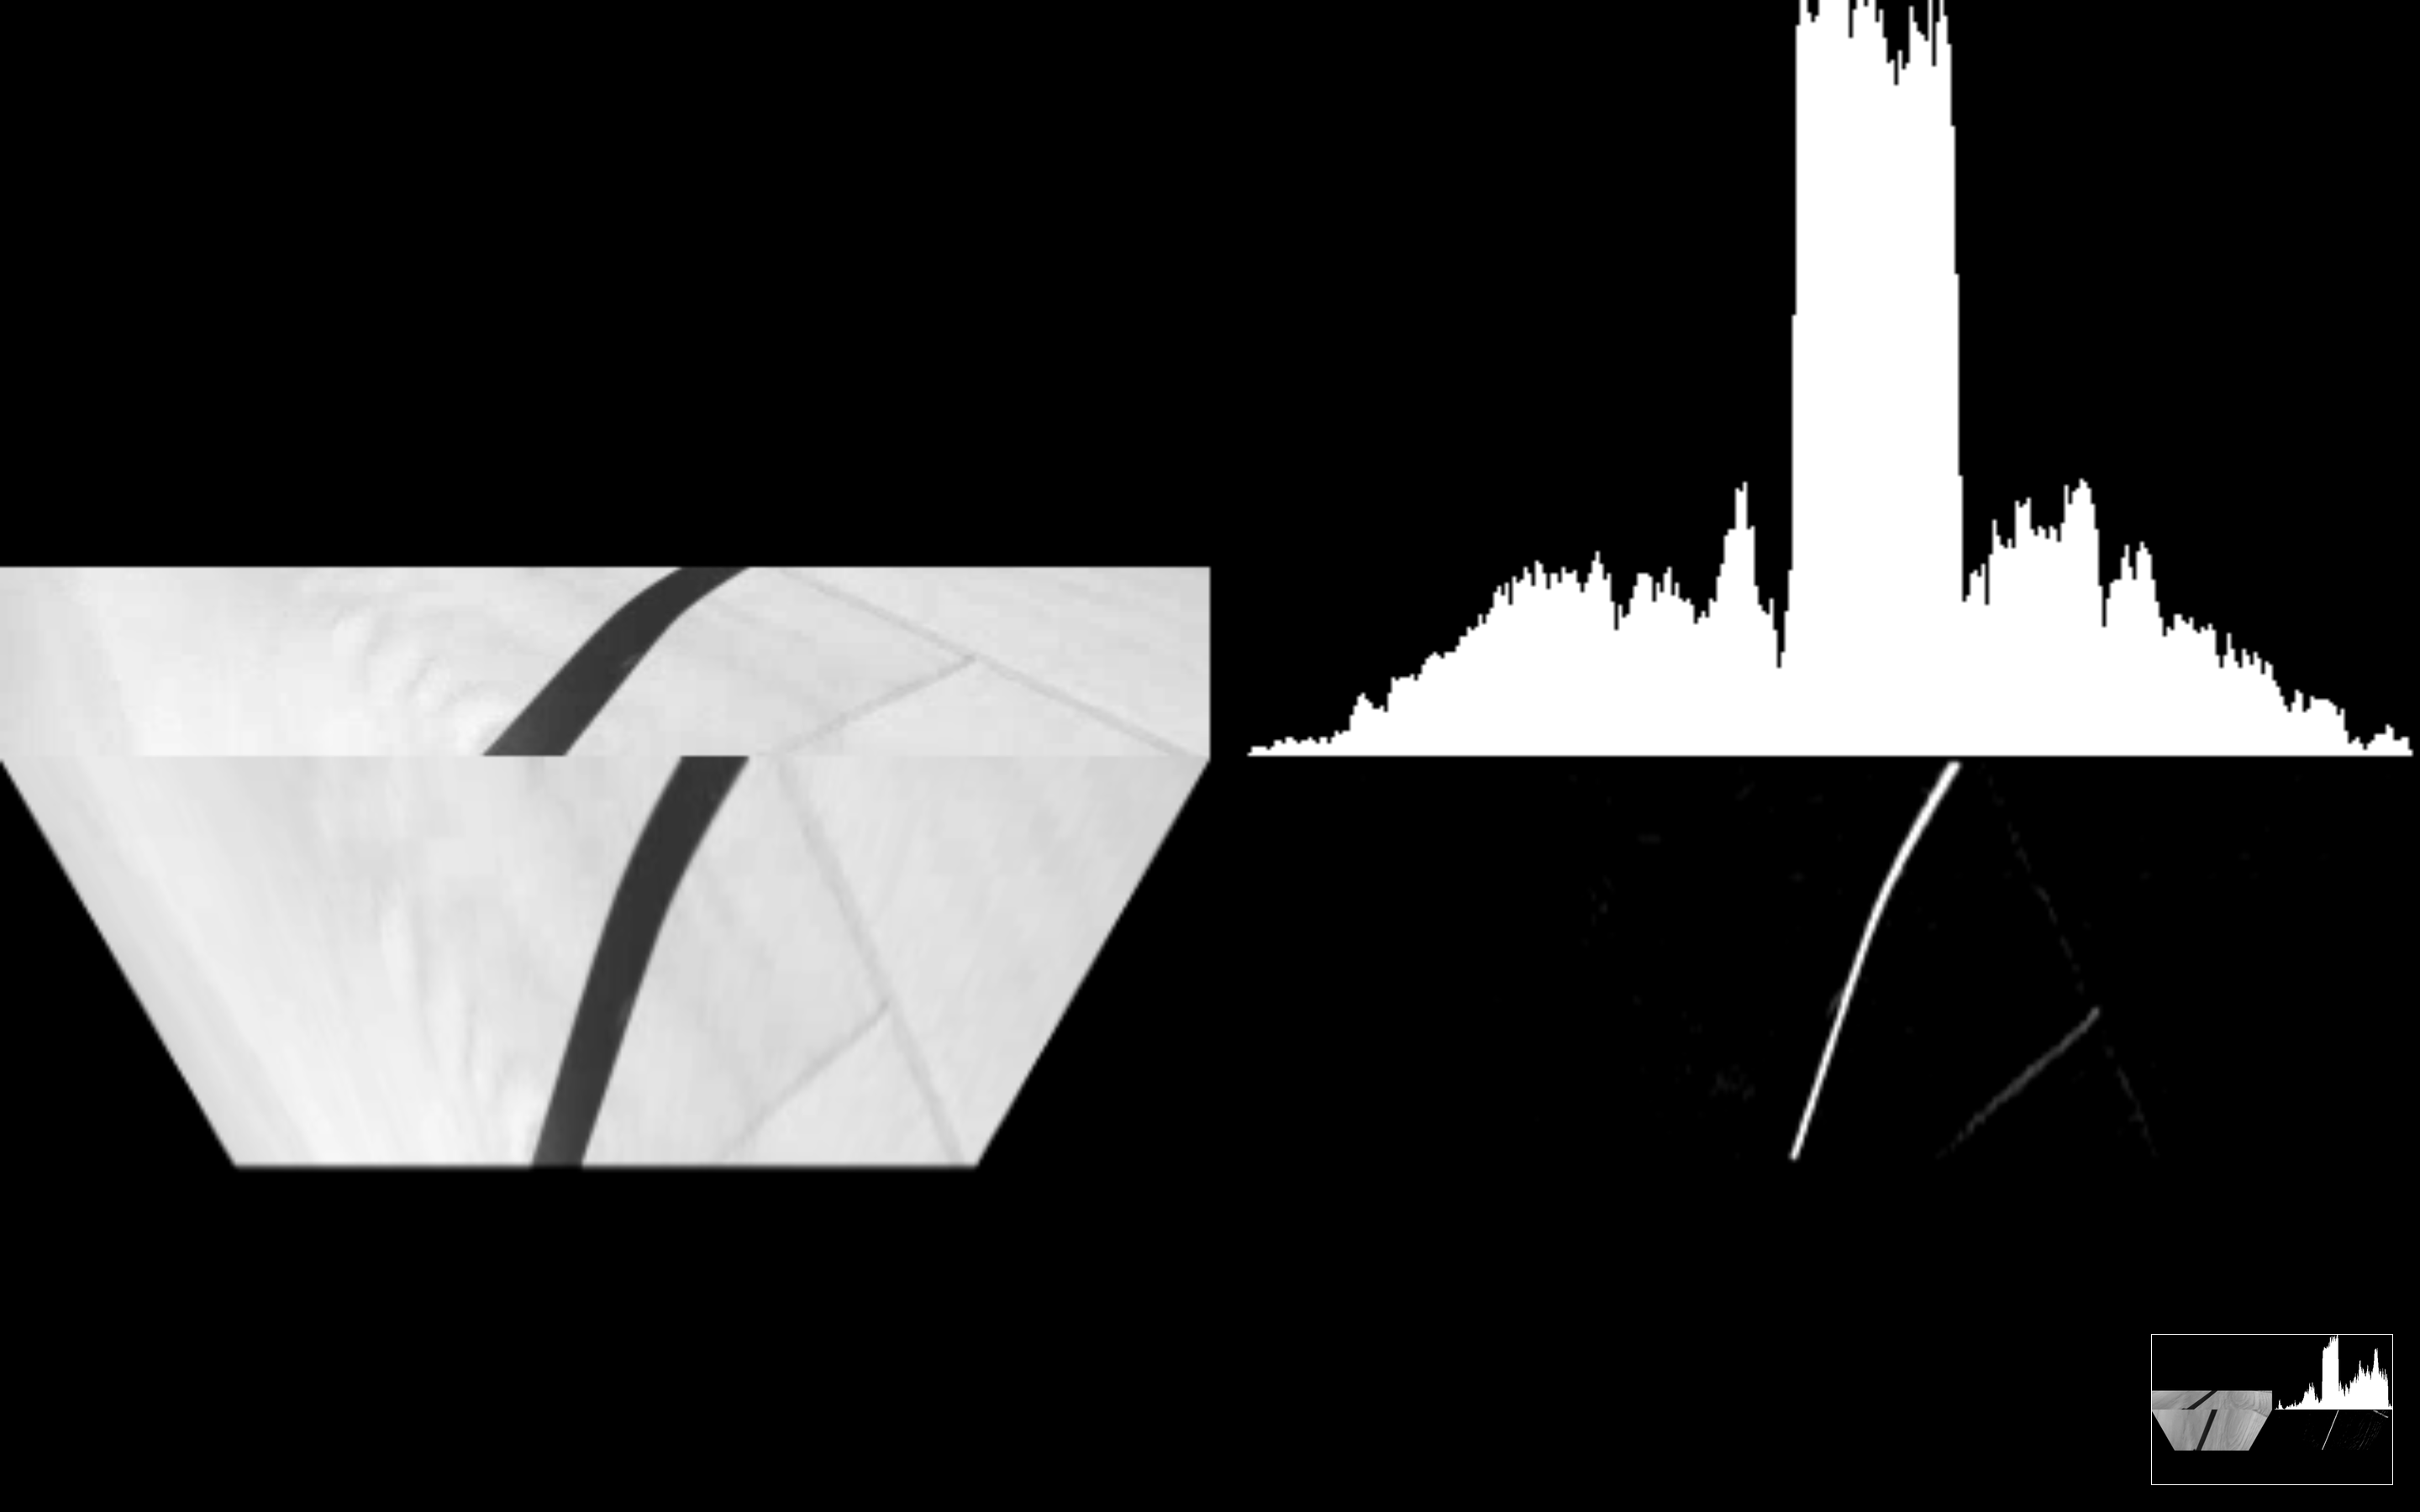
\includegraphics[width=\textwidth]{vizSmallCurve.png}
                \caption{Low Curvature}
                \label{fig:LineDetection}
            \end{subfigure}
            \hfill
            \begin{subfigure}[b]{0.45\textwidth}
                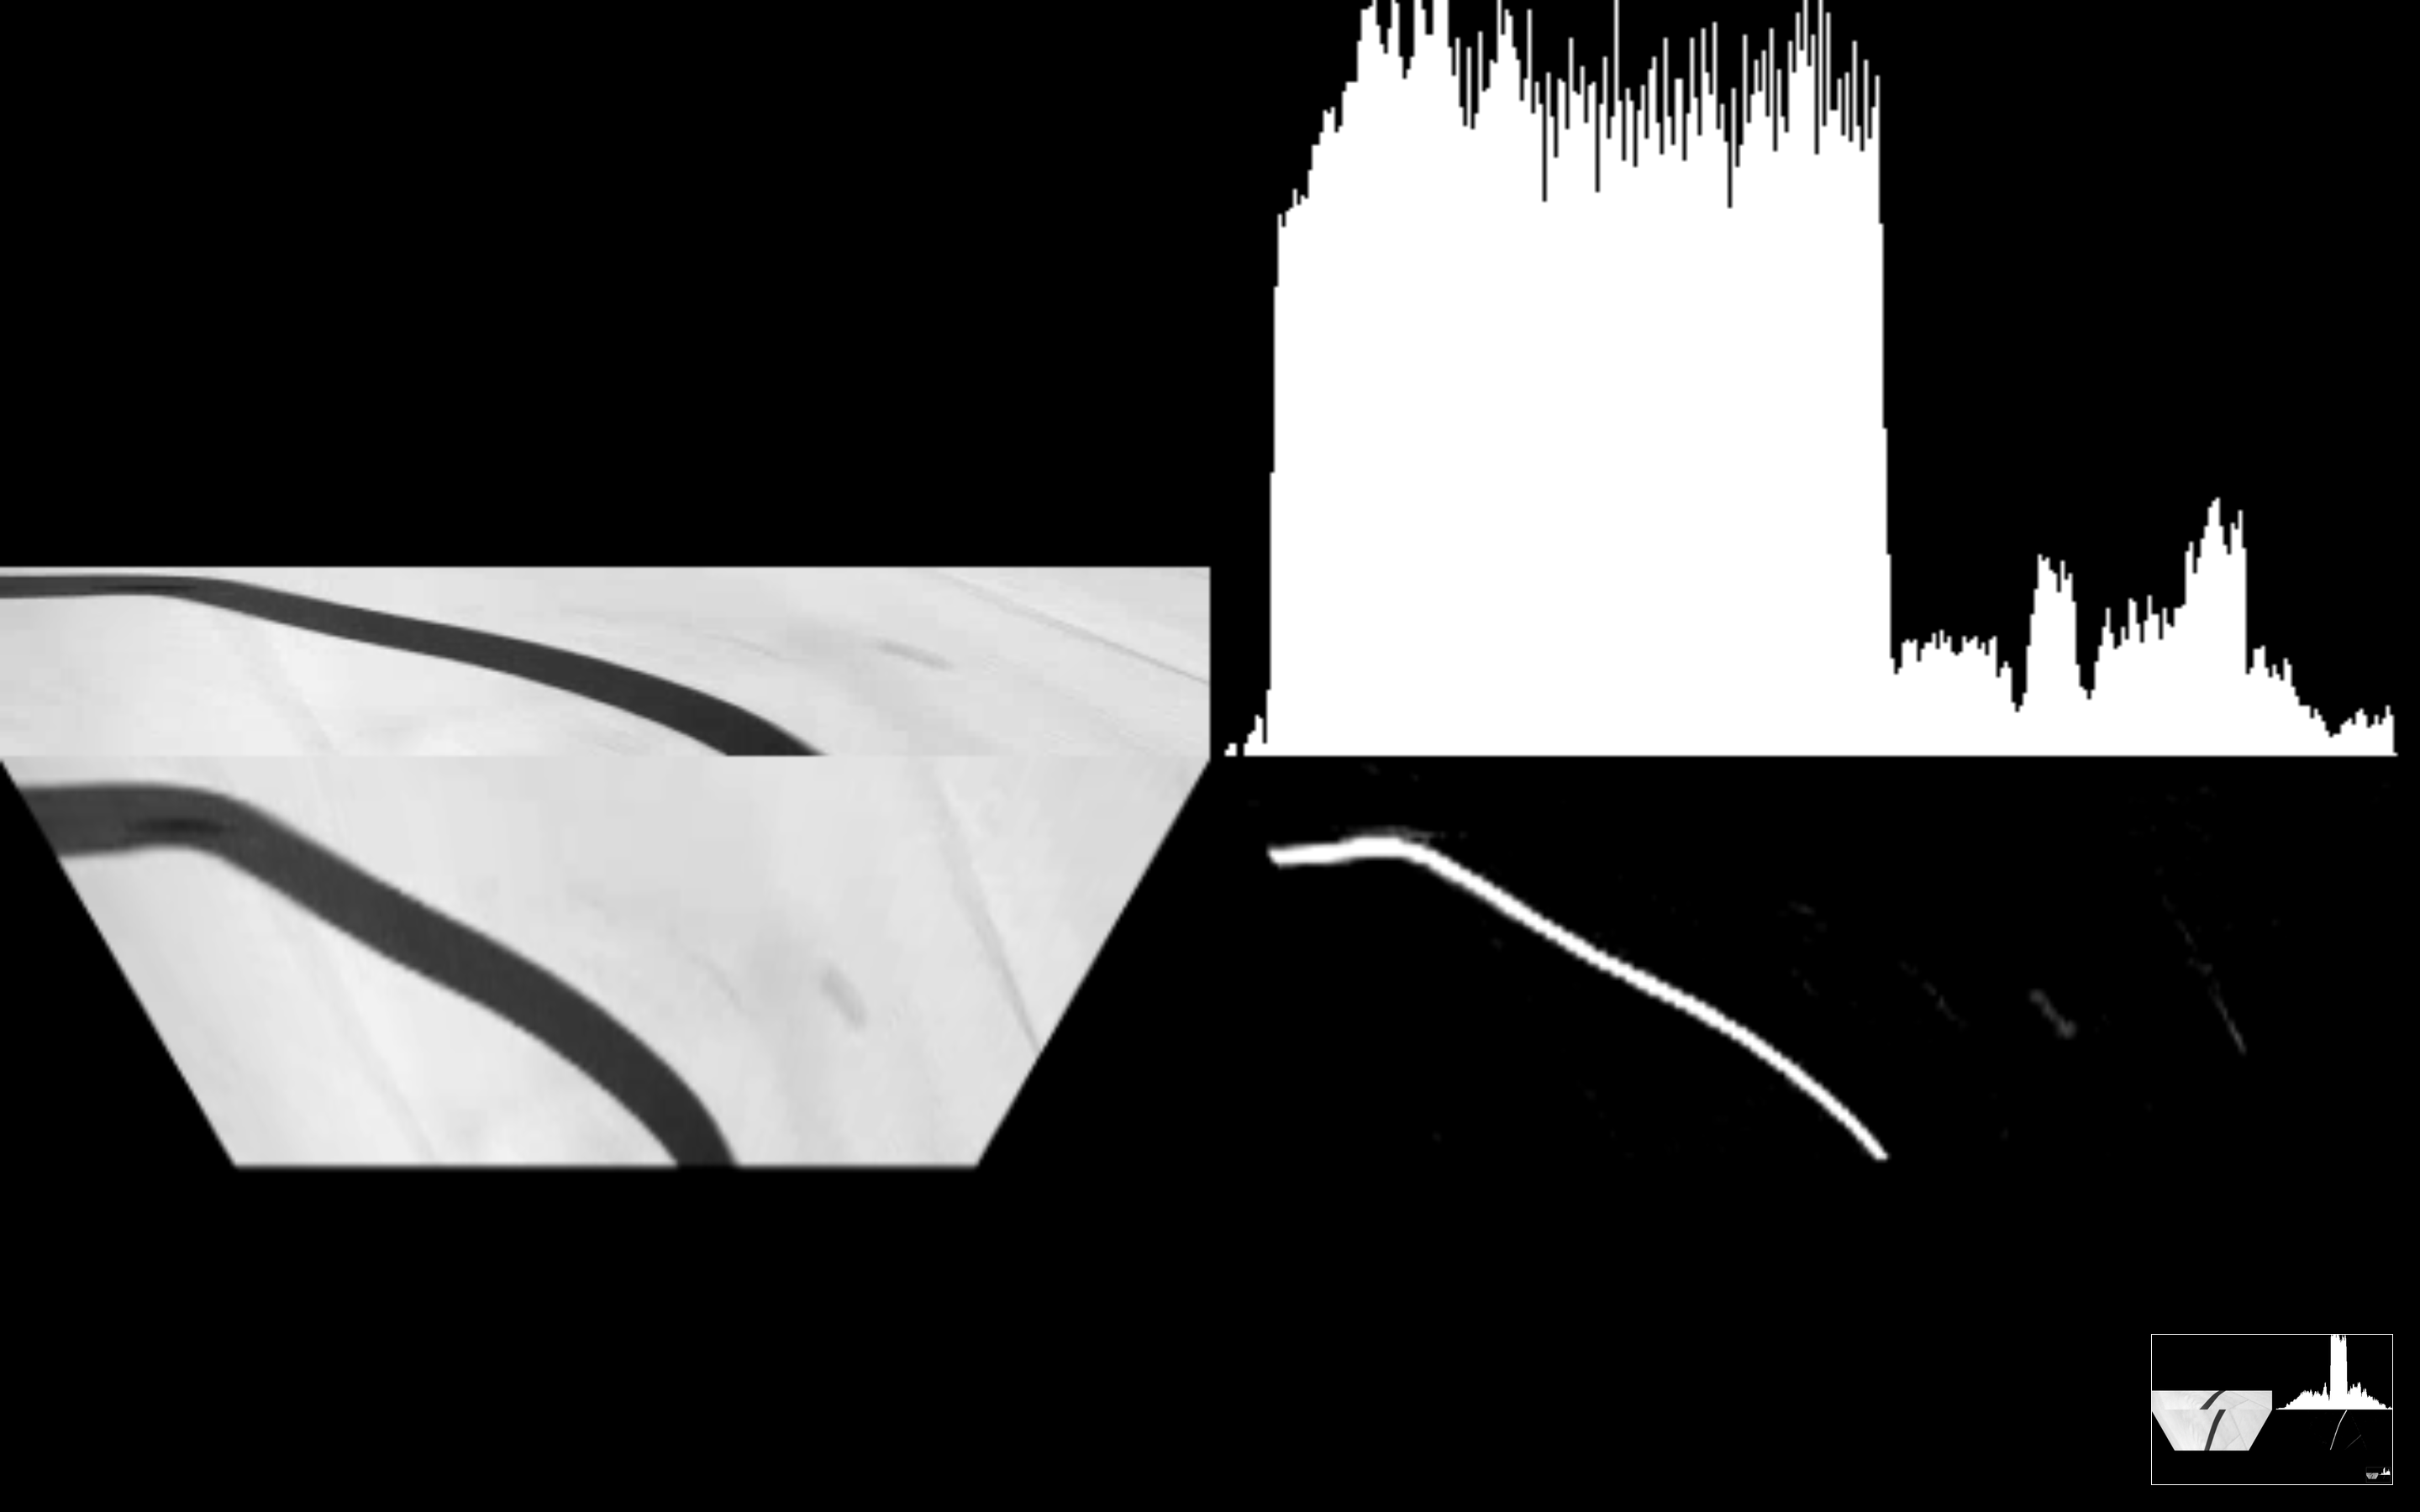
\includegraphics[width=\textwidth]{vizBigCurve.png}
                \caption{Sharp Curvature}
                \label{fig:LineSegmentation}
            \end{subfigure}
            \caption{Line Detection and Segmentation}   
        \end{figure}

        \begin{figure}[H]
            \centering
            \begin{subfigure}[b]{0.45\textwidth}
                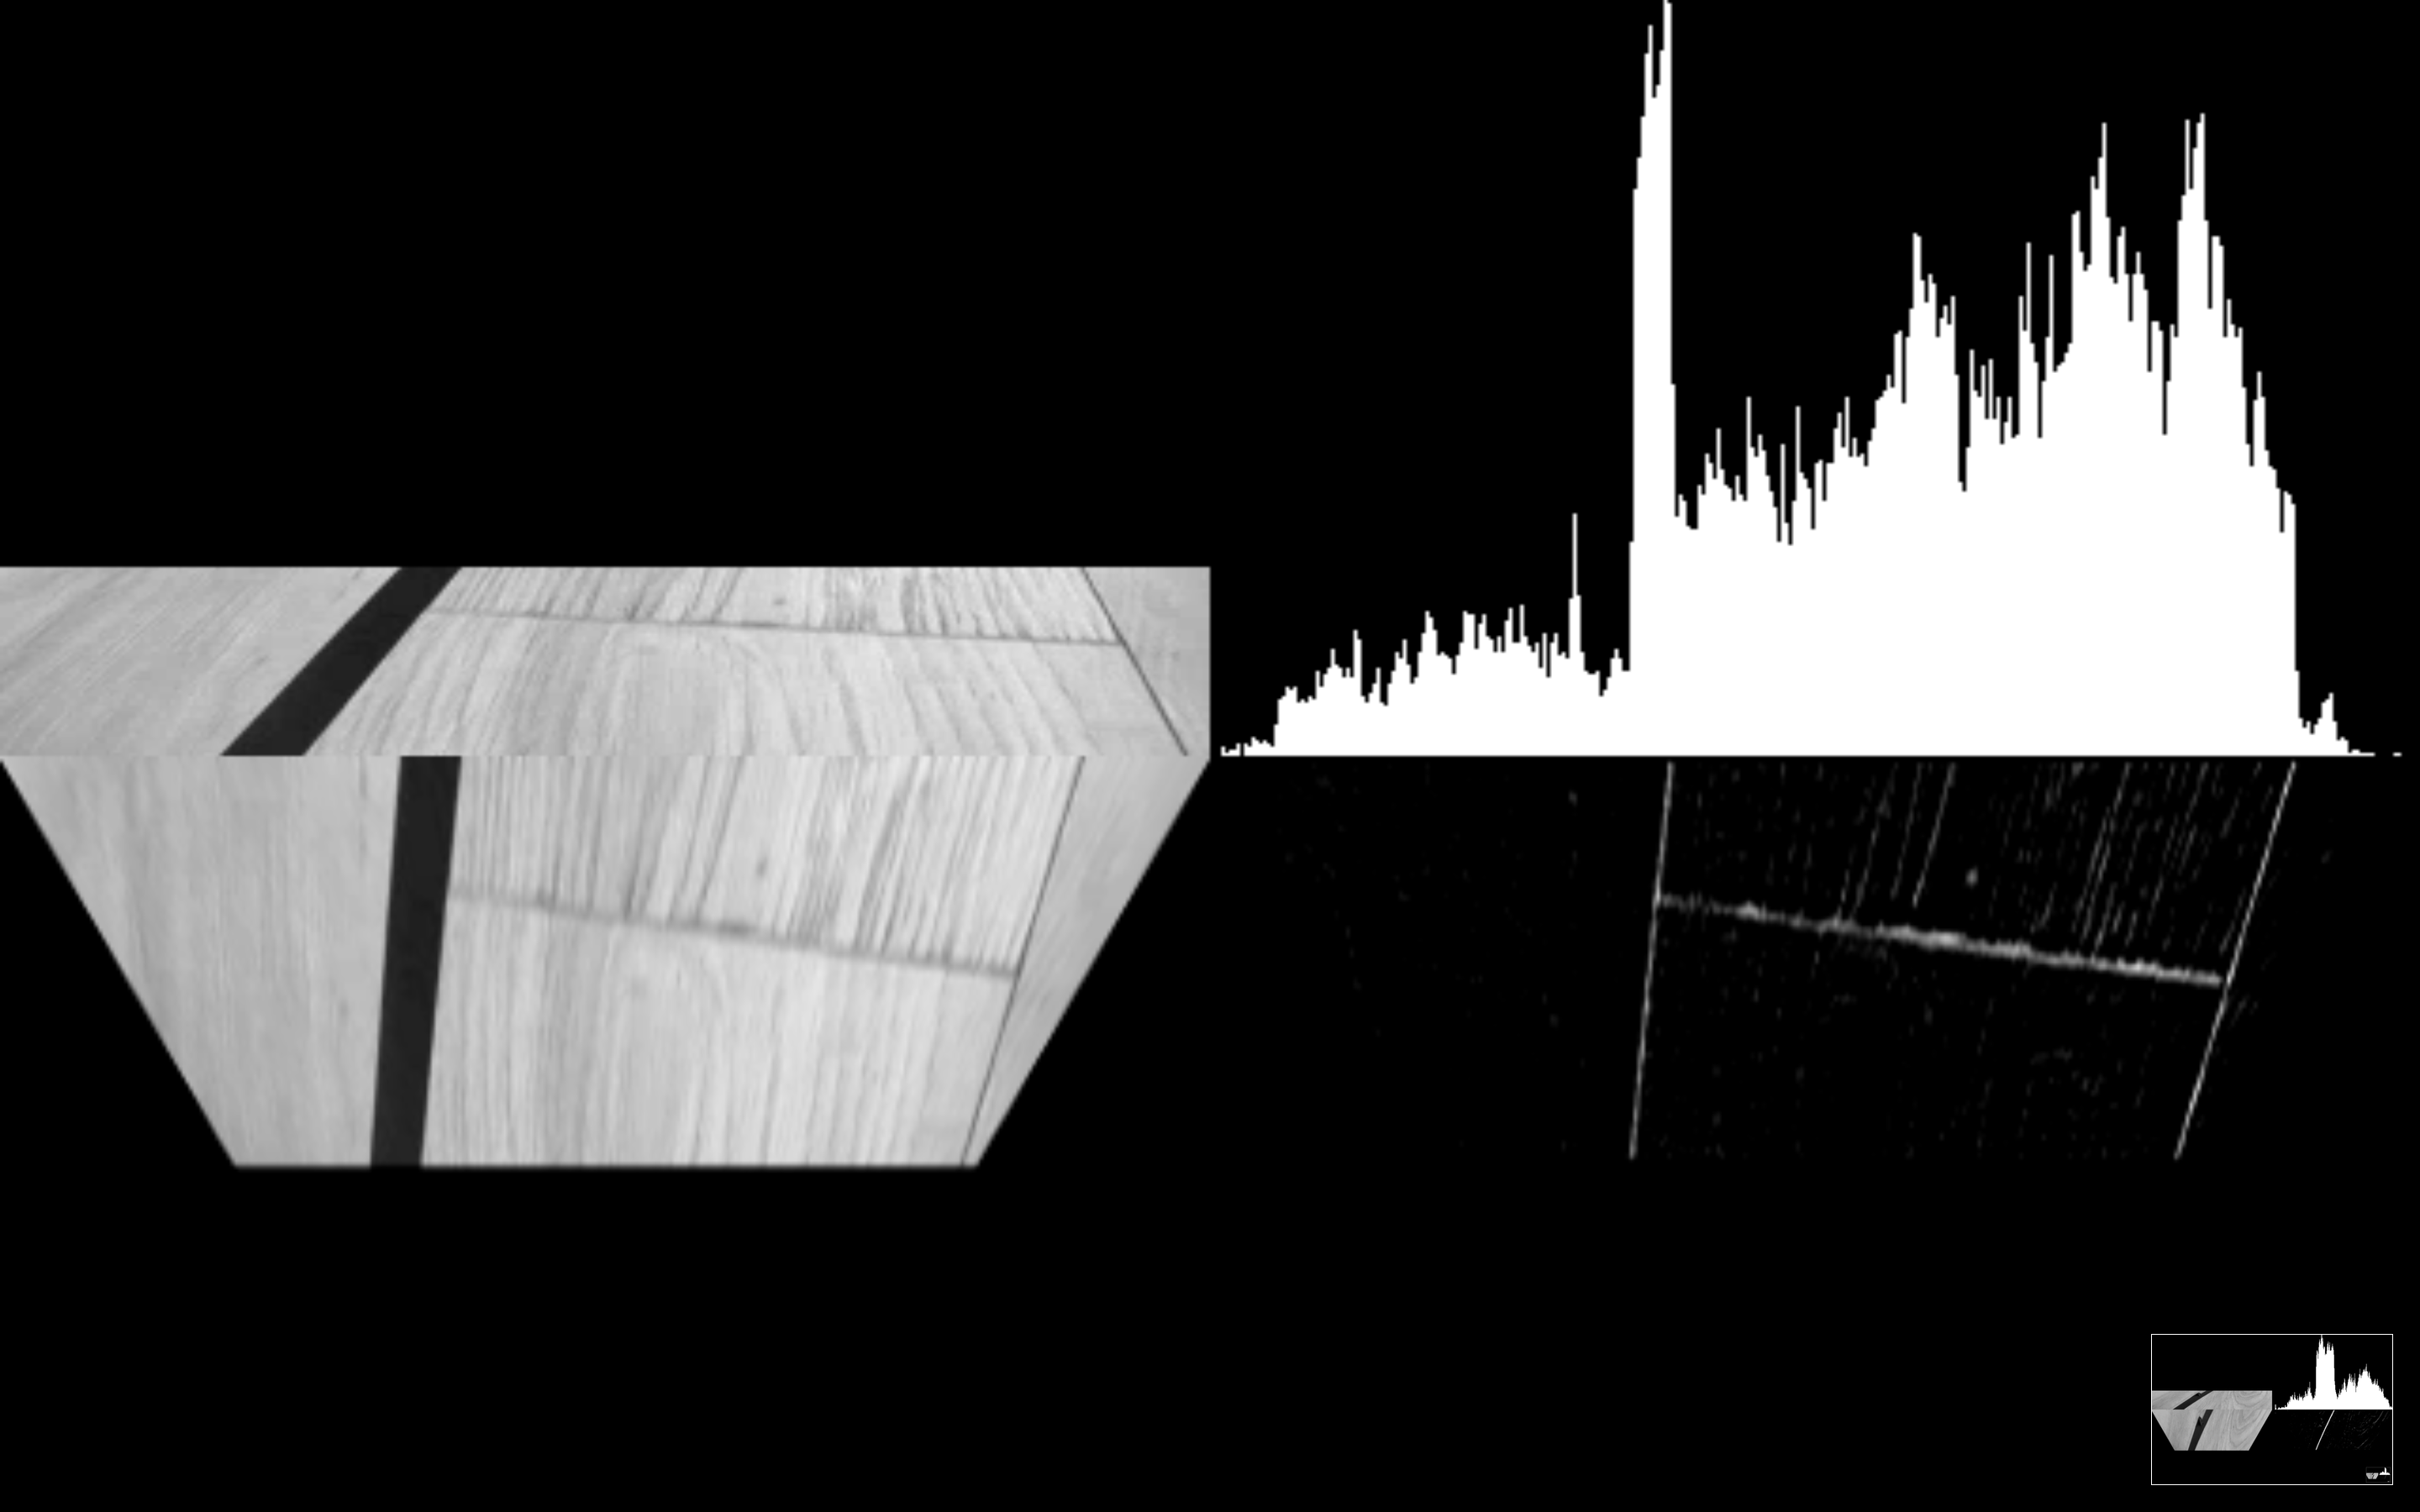
\includegraphics[width=\textwidth]{vizEnvNoise.png}
                \caption{False Positives}
                \label{fig:FalsePositives}
            \end{subfigure}
            \hfill
            \begin{subfigure}[b]{0.45\textwidth}
                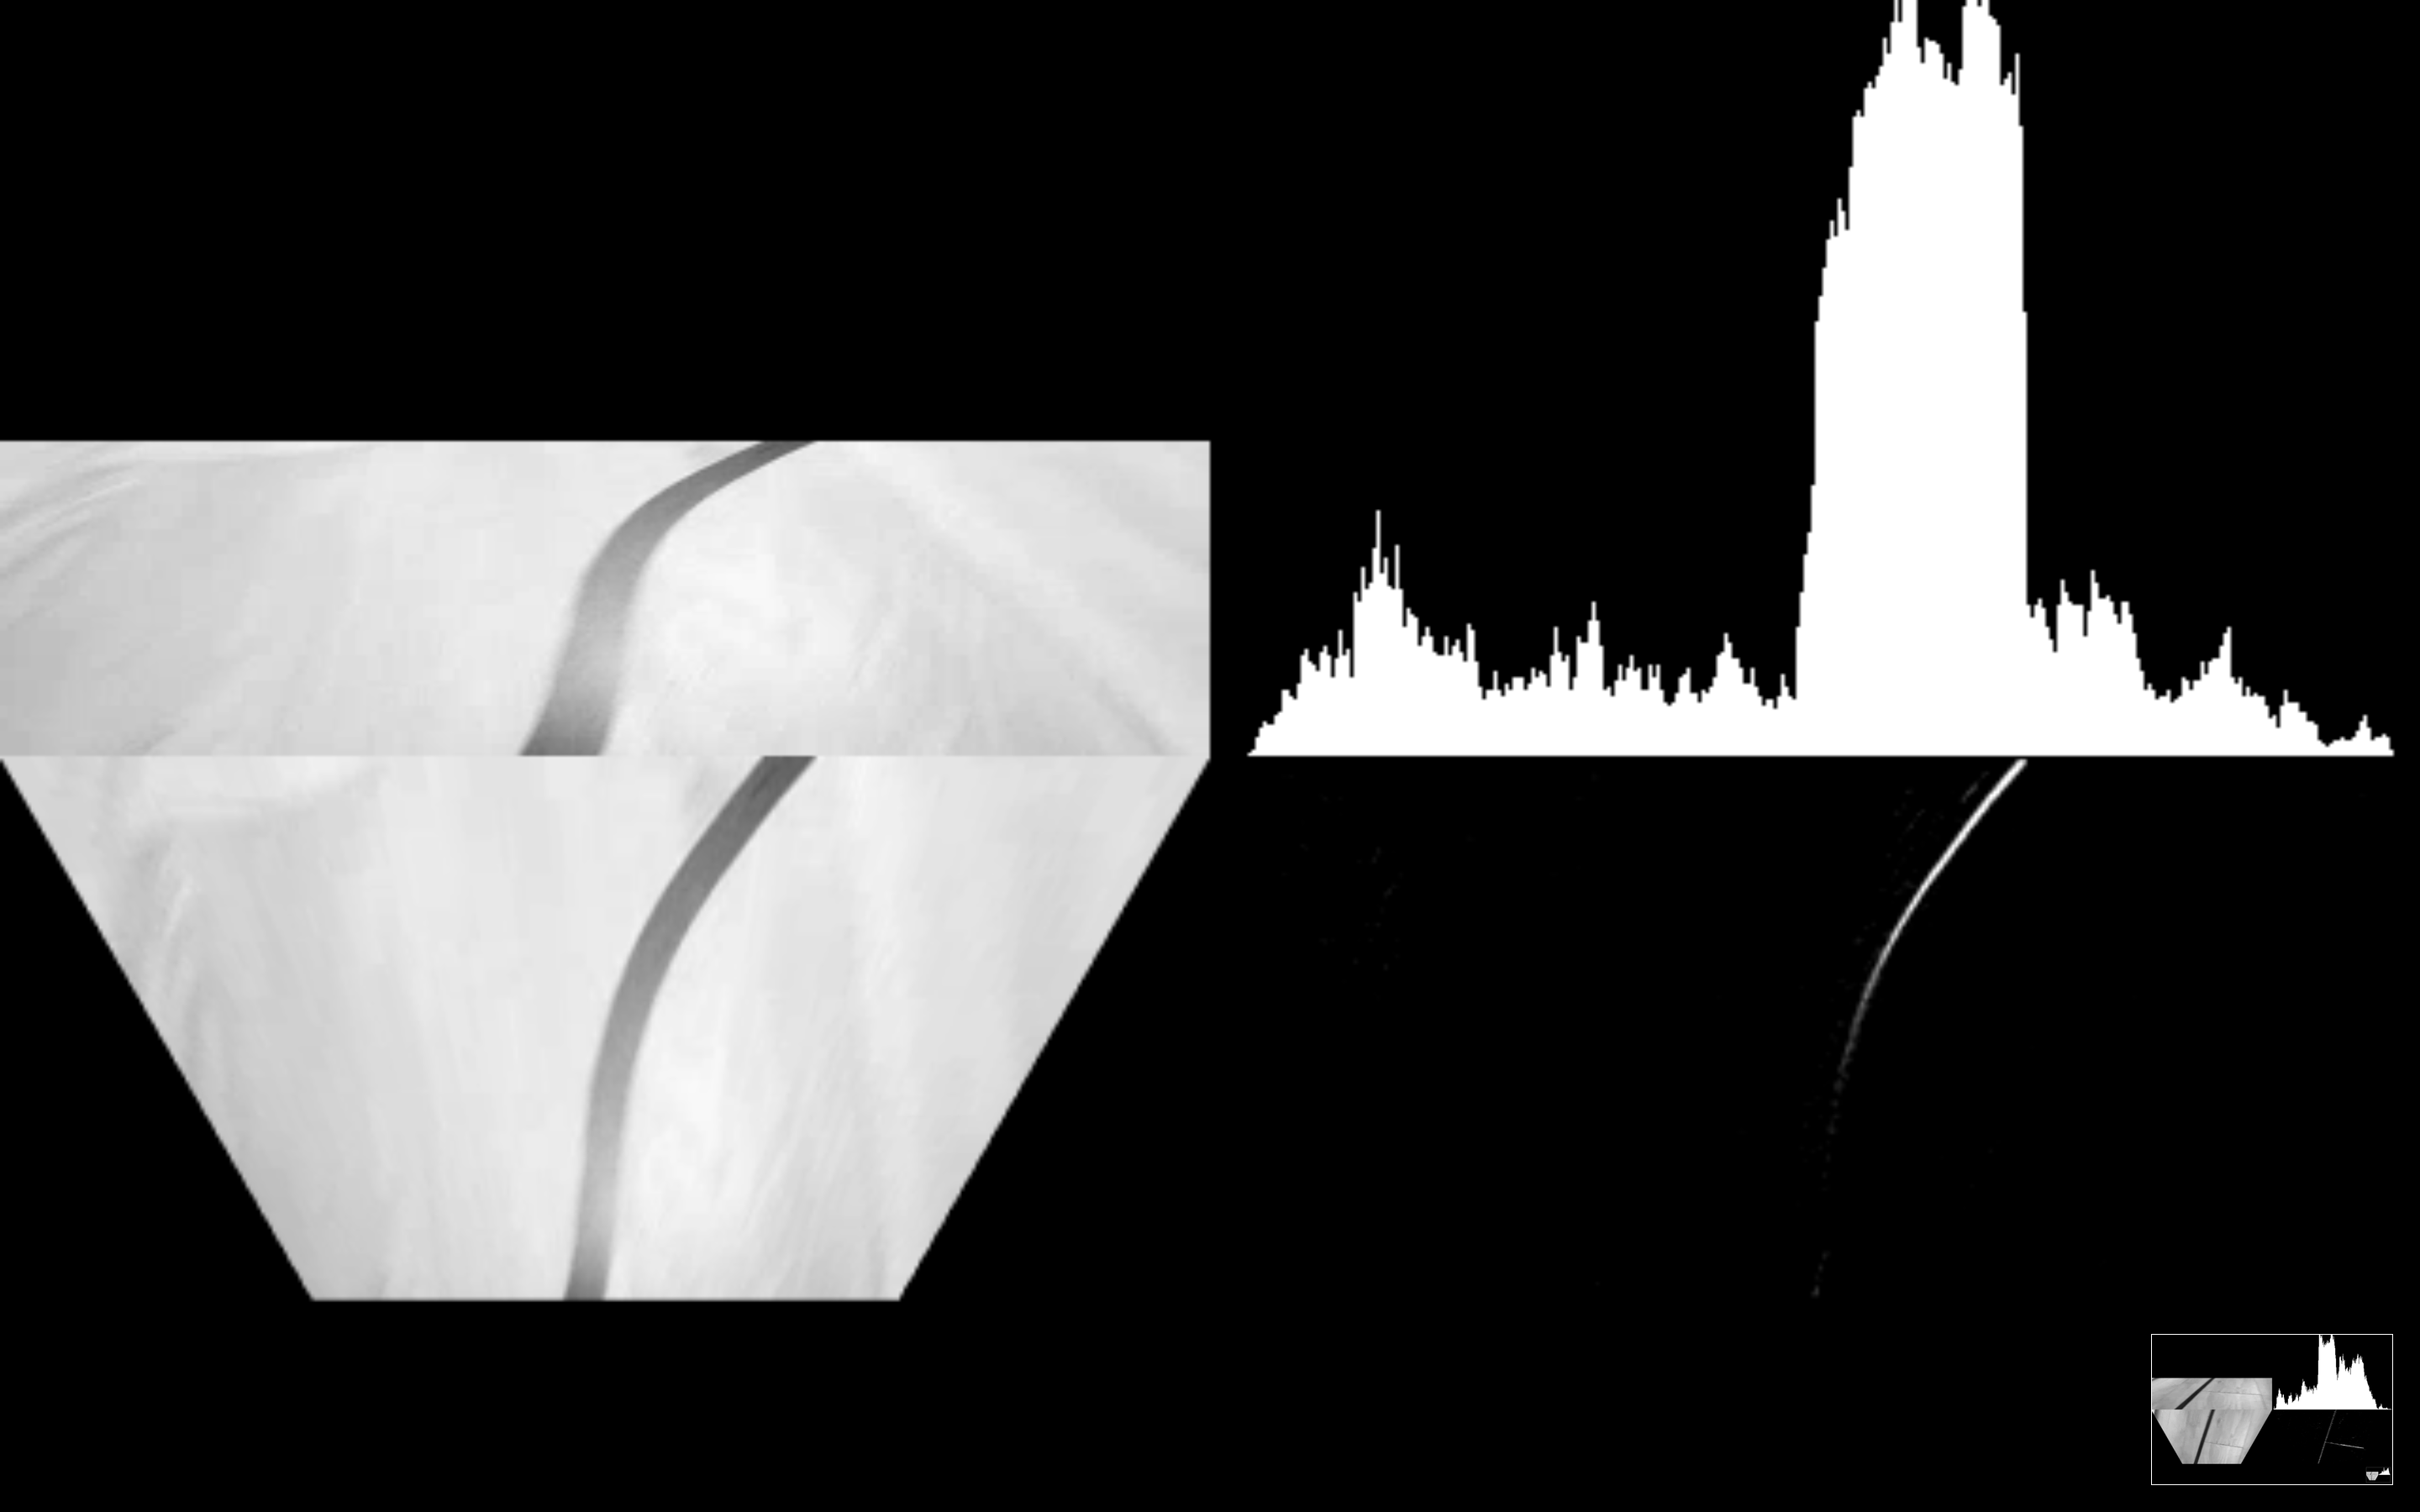
\includegraphics[width=\textwidth]{vizLightOclusion.png}
                \caption{Reflective Occlusion}
                \label{fig:ReflectOcclusion}
            \end{subfigure}
            \caption{Challenging Environments}
        \end{figure}

        \subsection{Navigation requirements}

        \subsection{Indoor Drivability Segmentation}

        \subsection{Racing Algorithms}

        \subsection{Predictive Trajectory Generation}
    
    \pagebreak{}


  %%%%%%%%%%%%%%%%%% SECTION 4 %%%%%%%%%%%%%%%%%%
  \section{Results and discussion} % edit section heading as appropriate
    \subsection{Balance Performance}

    \subsection{Operational Robustness}
    \subsection{Line Trajectory Tracking}
    \begin{figure}[H]
        \centering
        \begin{subfigure}[c]{0.35\textwidth}
            \includegraphics[height=1.3\textwidth]{Track.pdf}
            \caption{Race Track}
        \end{subfigure}
        \hfill
        \begin{subfigure}[c]{0.6\textwidth}
            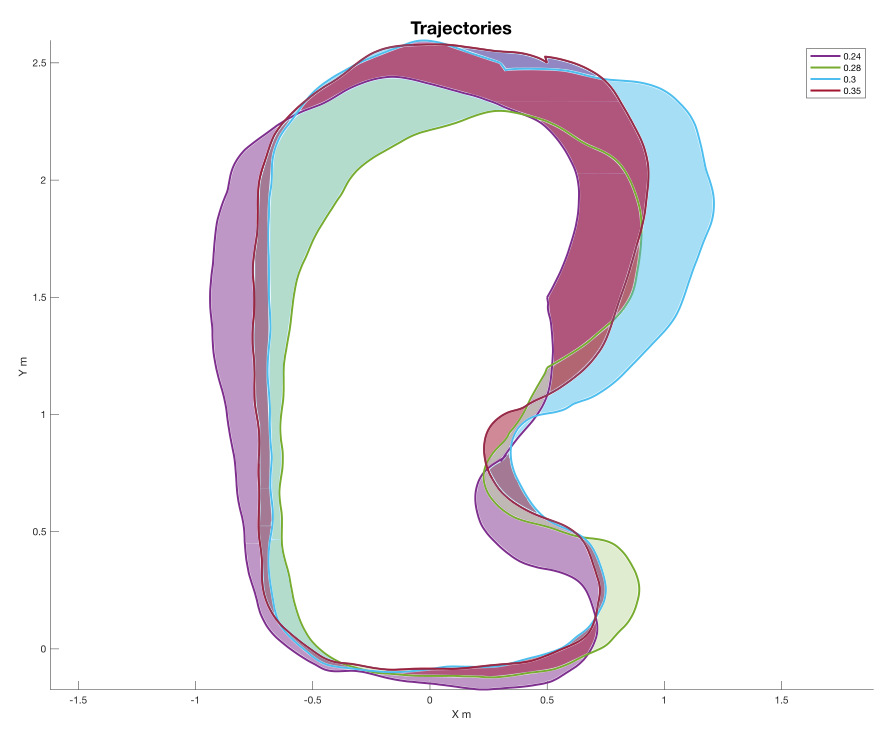
\includegraphics[width=\textwidth]{Graphs/DeadReckoningTrackMap.png}

            \caption{Map built offline using dead reckoning}
        \end{subfigure}
        \caption{Trajectory Tracking and Map Visualization}
        \label{fig:TrajTrack}
    \end{figure}
    \subsection{More detail}
    \subsection{Summary}
  %%%%%%%%%%%%%%%%%% SECTION 5 %%%%%%%%%%%%%%%%%%
  \section{Conclusions and future work} % edit section heading as appropriate
    \subsection{Conclusions}
      \subsection{Future work}
  %%%%%%%%%%%%%%%%%% REFERENCES %%%%%%%%%%%%%%%%%%
    \printbibliography
  %%%%%%%%%%%%%%%%%% APPENDICES %%%%%%%%%%%%%%%%%%
  \begin{uomappendix} 
      \section{Code}
      \section{Risk assessment}
      Risk assessment is a required appendix. Put here.
      %\section{Other appendices as necessary}
  \end{uomappendix}
  
  %%%%%%%%%%%%%%%%%% END MATTER %%%%%%%%%%%%%%%%%%
  \end{document}